% Created 2025-02-19 Wed 21:46
% Intended LaTeX compiler: pdflatex
\documentclass[11pt]{article}
\usepackage[utf8]{inputenc}
\usepackage[T1]{fontenc}
\usepackage{graphicx}
\usepackage{longtable}
\usepackage{wrapfig}
\usepackage{rotating}
\usepackage[normalem]{ulem}
\usepackage{amsmath}
\usepackage{amssymb}
\usepackage{capt-of}
\usepackage{hyperref}
\usepackage{minted}
\usepackage[margin=0.5in]{geometry}
\hypersetup{colorlinks, linkcolor=black}
\usepackage{geometry}
\geometry{top=2cm}
\geometry{bottom=2cm}
\usepackage{fancyhdr}
\pagestyle{fancy}
\fancyhf[L]{Servicios en Red e Internet}
\fancyhf[R]{Segunda Evaluación}
\fancyfoot[R]{ismael.macareno@educa.madrid.org}
\fancyfoot[L]{CC BY-NC-SA 4.0}
\usepackage{parskip}
\usepackage{mdframed}
\usepackage{fancyvrb}
\usepackage{xcolor}
\definecolor{shadecolor}{RGB}{220,220,220}
\newenvironment{shadedcode}{%
\VerbatimEnvironment
\begin{mdframed}[backgroundcolor=shadecolor,linewidth=0pt]}%
{\end{mdframed}}
\usepackage{attachfile2}
\newcommand{\textattachfilecolor}[2]{\textattachfile[color=0 0 0.5]{#1}{\textcolor{blue}{#2}}}
\usepackage[spanish]{babel}
\usepackage{datetime2}
\DTMlangsetup[es-ES]{ord=raise}
\renewcommand{\dateseparator}{/}
\usepackage{titlesec}
\usepackage{afterpage}
\newcommand\blankpage{\null\thispagestyle{empty}\newpage}
\usepackage{colortbl}
\usepackage{pdfpages}
\usepackage{tcolorbox}
\usepackage{listings}
\usepackage[spanish]{babel}
\lstset{
inputencoding=utf8,
extendedchars=true,
literate={ñ}{{\~n}}1 {Ñ}{{\~N}}1 {á}{{\'a}}1 {é}{{\'e}}1 {í}{{\'i}}1 {ó}{{\'o}}1 {ú}{{\'u}}1 {Á}{{\'A}}1 {É}{{\'E}}1 {Í}{{\'I}}1 {Ó}{{\'O}}1 {Ú}{{\'U}}1,
basicstyle=\ttfamily,
breaklines=true,
columns=fullflexible,
keepspaces=true,
language=TeX,
morekeywords={*, -, **, /}
}
\newtcolorbox[auto counter, number within=section]{alertblock}[2][]{colframe=red!75!black, colback=red!10!white, coltitle=black, fonttitle=\bfseries, title=#2,#1}
\author{Ismael Macareno Chouikh}
\date{\today}
\title{Apuntes Segunda Evaluación - SEREI}
\hypersetup{
 pdfauthor={Ismael Macareno Chouikh},
 pdftitle={Apuntes Segunda Evaluación - SEREI},
 pdfkeywords={},
 pdfsubject={},
 pdfcreator={Emacs 29.4 (Org mode 9.6.15)}, 
 pdflang={Spanish}}
\begin{document}

\maketitle
\tableofcontents

\blankpage

\section{FTP}
\label{sec:orga619a6c}
\subsection{vsftpd}
\label{sec:org4b8fe45}
\subsubsection{Instalación}
\label{sec:org6bbf7bc}
Para instalar cualquier tipo de paquete en una distribución Ubuntu tendremos que usar las siguientes instrucciones:
\begin{itemize}
\item \texttt{sudo apt-get update}
\item \texttt{sudo apt-get install vsftpd}
\end{itemize}


Podremos comprobar que el paquete está instalado mediante el uso de la instrucción \texttt{netstat -putona | grep -i vsftpd}

También se podrá comprobar accediendo desde nuestro navegador web a \texttt{ftp://localhost}

\begin{center}
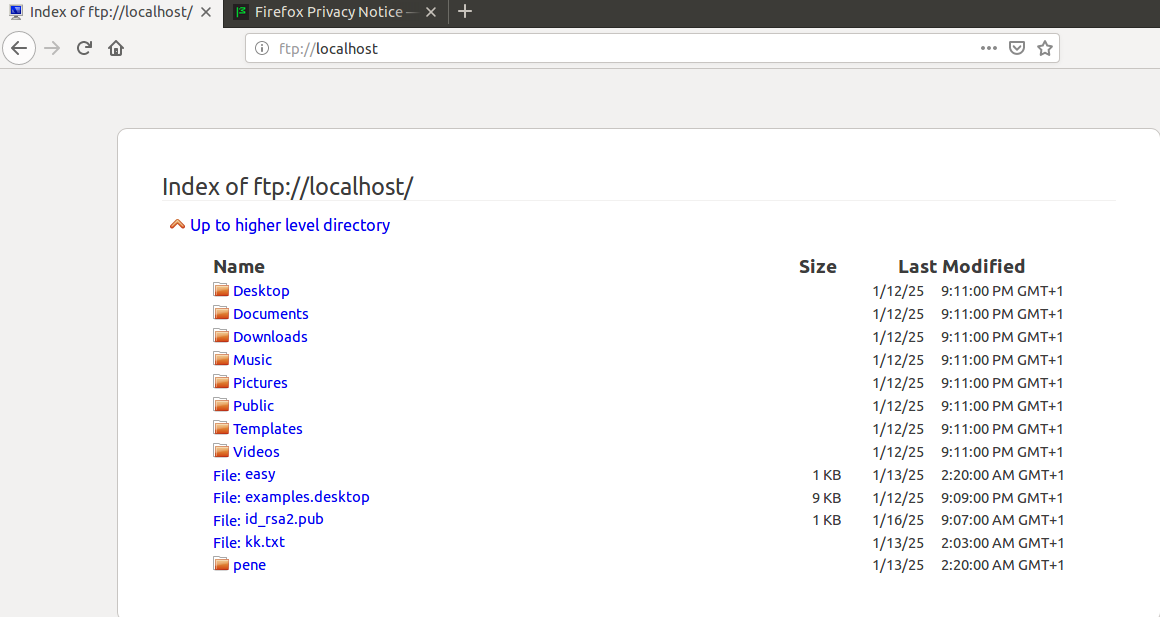
\includegraphics[width=.9\linewidth]{./media/ftp-1.png}
\end{center}

\subsubsection{Configuración}
\label{sec:org14e42e5}
Para configurar aspectos de \texttt{vsftpd} lo que tendremos que hacer será modificar el fichero \texttt{/etc/vsftpd.conf}

Como primera configuración lo que haremos será descomentar la línea 14 del fichero la cuál contiene \texttt{listen=YES} para que así cuando se inicie el sistema ftp se inicie con él.
\begin{minted}[,frame=single]{bash}
# daemon started from an initscript.
listen=YES
\end{minted}

Luego también descomentaremos las líneas 26, 29 y 33
\begin{minted}[,frame=single]{bash}
# Uncomment this to allow local users to log in.
local_enable=YES # Conexion con los usuarios locales del servidor
#
# Uncomment this to enable any form of FTP write command.
write_enable=YES # Los usuarios podrán escribir y descargar cosas
#
# Default umask for local users is 077. You may wish to change this to 022,
# if your users expect that (022 is used by most other ftpd's)
local_umask=022 # Los permisos de los ficheros subidos serán 755
\end{minted}

\subsubsection{\texttt{chroot}}
\label{sec:orgf569387}
Para habilitar el \texttt{chroot} lo que tendremos que hacer será descomentar la línea 120 del fichero \texttt{/etc/vsftpd.conf}
\begin{minted}[,frame=single]{bash}
chroot_local_user=YES
chroot_list_enable=YES
# (default follows)
chroot_list_file=/etc/vsftpd.chroot_list
\end{minted}

De esta manera conseguiremos enjaular a los usuarios, es decir, impedir el acceso a otras carpetas fuera del directorio de inicio de cada usuario.

\begin{itemize}
\item \texttt{chroot\_list\_enable=YES}: Permitir solo a ciertos usuario el poder navegar por todo el árbol de directorios del servidor
\item \texttt{chroot\_list\_file}: Estarán listados los usuarios que pueden navegar hacia arriba por los directorios del servidor.
\end{itemize}


A los usuarios que no queramos enjaular, los tendremos que meter en el fichero \texttt{/etc/vsftpd.chroot\_list}
\begin{minted}[,frame=single]{bash}
root@ubuntu2:~# cat /etc/vsftpd.chroot_list 
maka
\end{minted}

Para permitir la escritura tendremos que añadir la línea \texttt{allow\_writeable\_chroot=YES}

Para activar el modo pasivo para un máximo de 100 conexiones tendremos que añadir lo siguiente:
\begin{itemize}
\item \texttt{pasv\_enable=YES}
\item \texttt{pasv\_min\_port=40000}
\item \texttt{pasv\_max\_port=40100}
\end{itemize}


Luego de haber añadido esas tres líneas al fichero \texttt{/etc/vsftpd.chroot\_list} podremos reiniciar el servicio mediante la instrucción \texttt{service vsftpd restart} y seguidamente \texttt{ftp} escuchará por el
puerto 21.

\subsubsection{Grupos de usuario para \texttt{ftp}}
\label{sec:orga6e601e}
Los usuarios que se conectarán no tendrán acceso al servidor vía \texttt{SSH} o \emph{shell} local por lo tanto debemos darles permisos especiales.

Cuando se instala \texttt{vsftpd} se crea un grupo y usuario llamados \texttt{ftp} por defecto. Lo podremos verificar mediante la instrucción \texttt{egrep -i ftp /etc/group}

Ahora lo que haremos será habilitar una \emph{shell} fantasma para que los usuarios \texttt{ftp} no puedan entrar en la consola del servidor.

Para permitir el acceso del usuario \texttt{nologin} a una \emph{shell} fantasma lo que tendremos que hacer será modificar el fichero \texttt{/etc/shells} de tal manera que nos quede así:
\begin{minted}[,frame=single]{bash}
# /etc/shells: valid login shells
/bin/sh
/bin/dash
/bin/bash
/bin/rbash
/usr/bin/tmux
/usr/sbin/nologin
\end{minted}

\subsubsection{Crear usuarios para \texttt{ftp}}
\label{sec:orgc592f19}
Para los usuarios que pertenecerán al grupo ftp, crearemos la carpeta de los usuarios ftp en el servidor, será donde los usuarios ftp tendrán sus carpetas personales, todo en un directorio
raíz para facilitar la administración.
\begin{minted}[,frame=single]{bash}
root@ubuntu2:~# mkdir /home/usuariosftp
root@ubuntu2:~# chmod -R 777 /home/usuariosftp/
\end{minted}

Crear usuarios con el siguiente comando. Usa \emph{shell} \texttt{/usr/sbin/nologin} para evitar el acceso a la \emph{shell} para los usuarios ftp.

\begin{itemize}
\item \texttt{useradd -g ftp -d /home/usuariosftp/nombre  -m -s /usr/sbin/nologin -c «Nombre completo» nombre}
\end{itemize}

Los parámetros que usamos en la línea anterior son:
\begin{itemize}
\item \texttt{-g ftp}: el usuario pertence al grupo \texttt{ftp}
\item \texttt{-d /home/usuariosftp}: el directorio principal del usuario será \texttt{/home/usuariosftp/prueba}
\item \texttt{-m} para que se cree automáticamente el usuario prueba en el directorio dentro de la raíz \texttt{/home/usuariosftp/}
\item \texttt{-s /usr/sbin/nologin}: el usuario no tendrá acceso a la \emph{shell} del sistema, así no podrá iniciar sesión en el servidor (solo acceso \texttt{ftp})
\item \texttt{-c "Prueba usuarios"}: el nombre completo del usuario
\item \texttt{prueba}: la última palabra será el nombre del usuario
\end{itemize}


Ahora lo que tendremos que hacer será crear la contraseña para el usuario \texttt{prueba} mediante el uso de la instrucción \texttt{passwd}
\begin{minted}[,frame=single]{bash}
root@ubuntu2:~# passwd prueba
Enter new UNIX password: 
Retype new UNIX password: 
passwd: password updated successfully
\end{minted}

Luego de todo el procedimiento de haber creado los usuario lo que podremos hacer será comprobar que de verdad todo está bien configurado tal y como deseamos.

La primera comprobación la haré desde un cliente \emph{Windows 10 LTSC} usando el programa Filezilla cliente.

\begin{center}
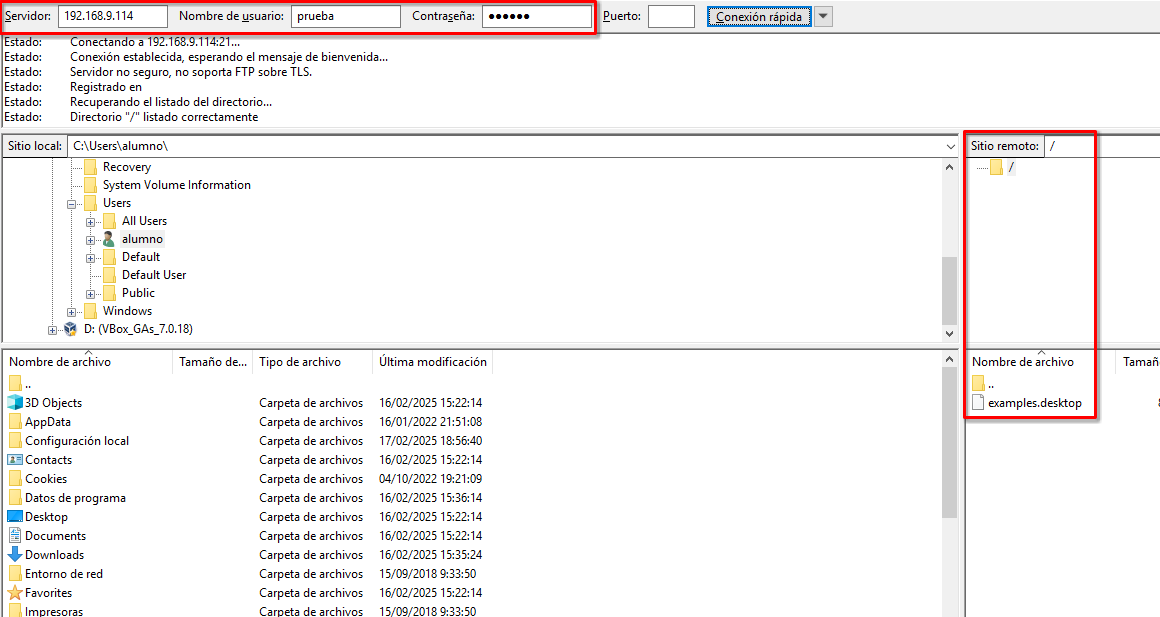
\includegraphics[width=.9\linewidth]{./media/ftp-2.png}
\end{center}

Este usuario no puede iniciar sesión a la consola como dicen las directivas \texttt{nologin}
\begin{minted}[,frame=single]{bash}
root@ubuntu2:~# su - prueba
This account is currently not available.
\end{minted}

Ahora probaré a conectarme mediante \emph{Filezilla client} pero a otro usuario el cuál no está enjaulado

\begin{center}
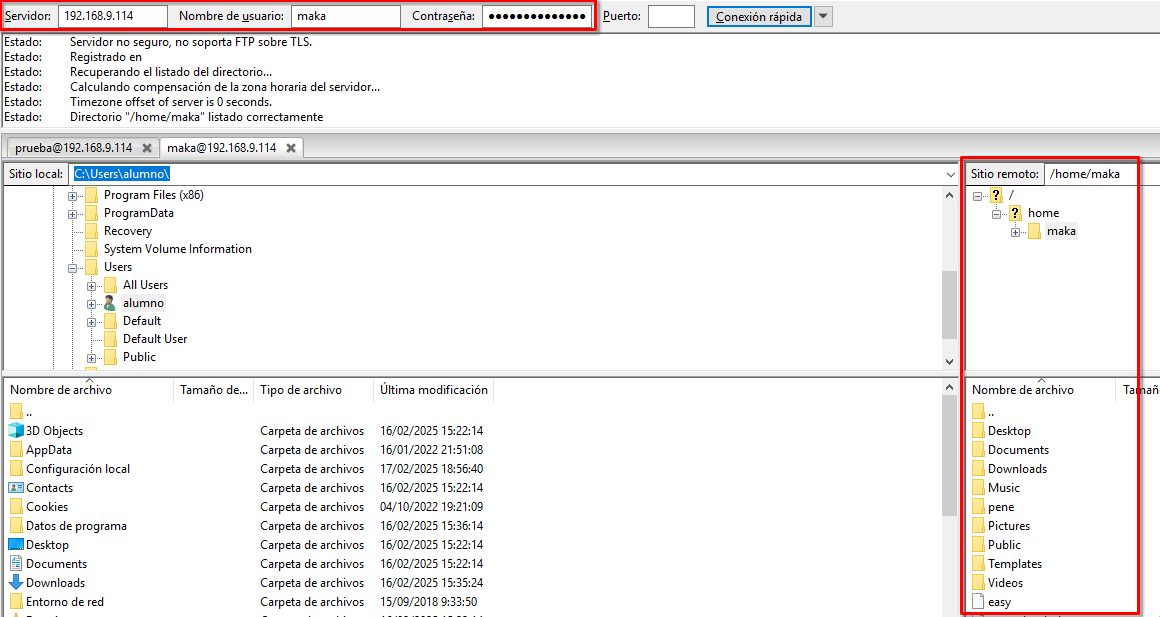
\includegraphics[width=.9\linewidth]{./media/ftp-3.png}
\end{center}

\subsubsection{Usuario anónimo}
\label{sec:org695b1ef}
Para habilitar el usuario \texttt{anonymous} lo que tendremos que hacer será modificar el fichero \texttt{/etc/vsftpd.conf} descomentando la línea que contenga \texttt{anonymous\_enable=YES} de la siguiente manera:
\begin{minted}[,frame=single]{bash}
# Allow anonymous FTP? (Disabled by default)
anonymous_enable=YES
\end{minted}

después de haber descomentado esa línea lo que tendremos que hacer será reiniciar el servicio mediante la instrucción \texttt{sudo service vsftpd restart} y ya podremos conectarnos usando el usuario
\texttt{anonymous}
\begin{minted}[,frame=single]{bash}
C:\Users\alumno>ftp 192.168.9.114
Conectado a 192.168.9.114.
220 (vsFTPd 3.0.2)
200 Always in UTF8 mode.
Usuario (192.168.9.114:(none)): anonymous
331 Please specify the password.
Contraseña:
230 Login successful.
ftp>
\end{minted}
\subsection{FTP sobre SSL}
\label{sec:org4c8b3cf}
Si solemos usar el protocolo \texttt{FTP} y no queremos que nos saquen contraseñas o directamente los ficheros que no pasen sin encriptación entre un servidor y un cliente, para ello debemos
habilitar la capa segura o SSL.

\texttt{FTP} en el puerto 21 es un gran riesgo para la seguridad porque con un analizador de paquetes TCP (Ej. \emph{wireshark}), primero haré un esnifado para comprobar que el usuario y la contraseña
viaja por la red en texto plano y los ficheros que enviemos también.

\begin{center}
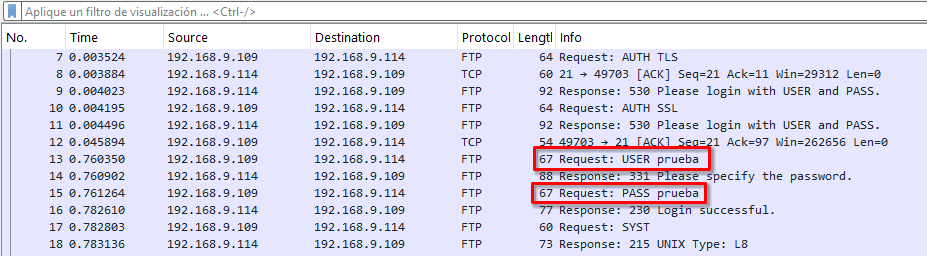
\includegraphics[width=.9\linewidth]{./media/ftp-4.png}
\end{center}

\subsubsection{Integrar seguridad \texttt{SSL} a \texttt{FTP}}
\label{sec:org18ccc30}
Habrá que crear un directorio para almacenar los certificados \texttt{ssl}. Usaremos la instrucción \texttt{sudo mkdir -p /etc/ssl/private}

Luego tendremos que dar permisos a \texttt{root} para ese directorio mediante la instrucción \texttt{sudo chmod 700 /etc/ssl/private}
\begin{minted}[,frame=single]{bash}
root@ubuntu2:~# mkdir -p /etc/ssl/private/
root@ubuntu2:~# chmod -R 700 /etc/ssl/private/
\end{minted}

\subsubsection{Generar un certificado \texttt{SSL} para \texttt{FTP}}
\label{sec:org087fa4d}
Habrá que estar conectado con el usuario \texttt{root} ya que solo él tiene permisos a el directorio donde se almacena la clave \texttt{ssl}.

Luego habrá que ejecutar la siguiente instrucción:
\begin{itemize}
\item \texttt{openssl req -x509 -nodes -days 365 -newkey rsa:4096 -keyout /etc/ssl/private/vsftpd.pem -out /etc/ssl/private/vsftpd.pem}
\end{itemize}


Y rellenar los campos de la siguiente manera:
\begin{minted}[,frame=single]{bash}
root@ubuntu2:~# openssl req -x509 -nodes -days 365 -newkey rsa:4096 -keyout /etc/ssl/private/vsftpd.pem -out /etc/ssl/private/vsftpd.pem
Generating a 4096 bit RSA private key
...............................................................++
..................++
writing new private key to '/etc/ssl/private/vsftpd.pem'
-----
You are about to be asked to enter information that will be incorporated
into your certificate request.
What you are about to enter is what is called a Distinguished Name or a DN.
There are quite a few fields but you can leave some blank
For some fields there will be a default value,
If you enter '.', the field will be left blank.
-----
Country Name (2 letter code) [AU]:ES
State or Province Name (full name) [Some-State]:MADRID
Locality Name (eg, city) []:ALCALA DE HENARES
Organization Name (eg, company) [Internet Widgits Pty Ltd]:IES Alonso de Avellaneda
Organizational Unit Name (eg, section) []:ASIR
Common Name (e.g. server FQDN or YOUR name) []:asir.iesavellaneda.com
Email Address []:ismael.macareno@educa.madrid.org
\end{minted}

Por último tendremos que modificar el fichero \texttt{/etc/vsftpd.conf} de tal manera que contenga las siguientes líneas:
\begin{itemize}
\item \texttt{ssl\_enable=YES}: habilitar \texttt{ssl}
\item \texttt{allow\_anon\_ssl=YES}: permite al usuario anónimo usar \texttt{ssl}
\item \texttt{force\_local\_data\_ssl=YES}: forzar a los usuarios ftp a usar \texttt{ssl}
\item \texttt{force\_local\_login\_ssl=YES}: forzar a los usuarios local a usar \texttt{ssl}
\item \texttt{ssl\_tlsv1=YES}: habilitar ssl v1
\item \texttt{ssl\_sslv2=NO}: no permitir ssl por seguridad
\item \texttt{ssl\_sslv3=NO}: no permitir ssl por seguridad
\item \texttt{rsa\_cert\_file=/etc/ssl/private/vsftpd.pem}: definir la ruta donde esta el certificado
\end{itemize}


\begin{minted}[,frame=single]{bash}
# This option specifies the location of the RSA certificate to use for SSL
# encrypted connections.
rsa_cert_file=/etc/ssl/private/vsftpd.pem
# This option specifies the location of the RSA key to use for SSL
# encrypted connections.
rsa_private_key_file=/etc/ssl/private/vsftpd.pem

# Habilitar escribir a los usuarios enjaulados
allow_writeable_chroot=YES

#Certificado SSL
ssl_enable=YES
allow_anon_ssl=YES
force_local_data_ssl=YES
force_local_logins_ssl=YES
ssl_tlsv1=YES
ssl_sslv2=NO
## Compatibilidad
ssl_sslv3=NO
require_ssl_reuse=NO
ssl_ciphers=HIGH
\end{minted}

Guardamos el fichero y reiniciamos el servicio mediante la instrucción \texttt{sudo service vsftpd restart}

Ahora vamos con las comprobaciones, si intentamos conectarnos desde nuestro Filezilla cliente se rechaza la conexión por los usuarios \texttt{ftp} pero permite los anónimos.

Para conectarnos desde un usuario autenticado tendremos que habilitar \texttt{SSL} en el \emph{software} de Fillezila cliente. Para ello en Filezilla iremos a:
\begin{enumerate}
\item Sitio nuevo
\item Habilitar TLS
\item Rellenaremos los datos para conectarnos
\end{enumerate}

\begin{center}
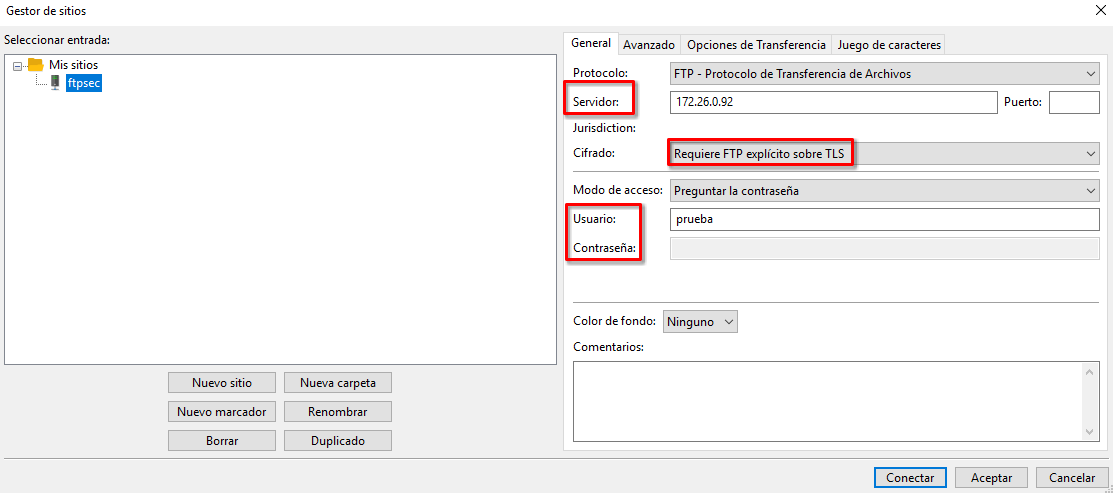
\includegraphics[width=.9\linewidth]{./media/ftp-5.png}
\end{center}

\begin{center}
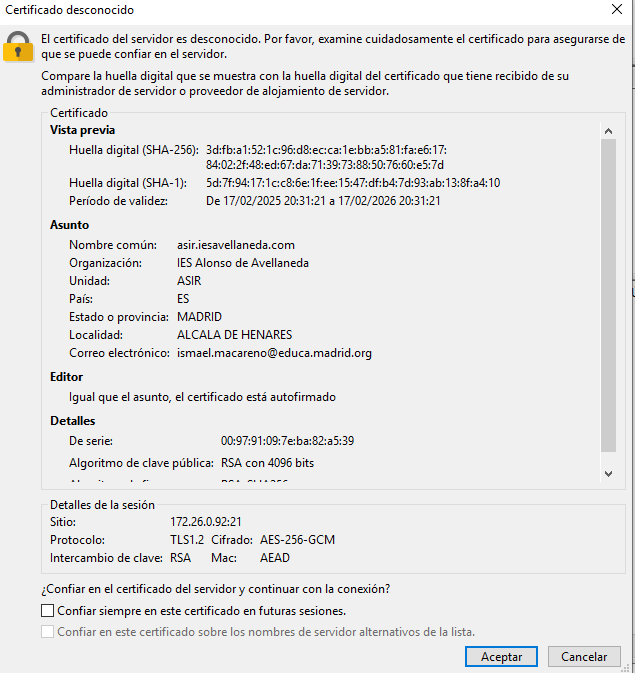
\includegraphics[width=.9\linewidth]{./media/ftp-6.png}
\end{center}

\subsection{\emph{Filezilla Server}}
\label{sec:org5ac565b}
\subsubsection{Instalación de \emph{Filezilla Server}}
\label{sec:org30e7356}
Necesitaremos una máquina virtual \emph{Windows Server 2016 Datacenter}.

Cuando tengamos la máquina virtual \emph{Windows} lo que haremos será descargar un \texttt{.exe} de la versión \emph{Filezilla server 0.9.51} y ejecutarlo para instalar.

\begin{figure}[htbp]
\centering
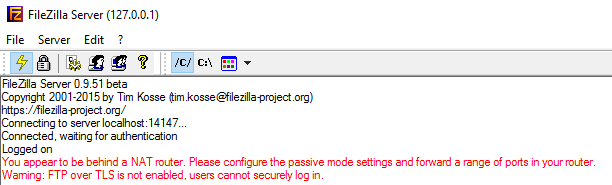
\includegraphics[width=.9\linewidth]{./media/1.png}
\caption{Macareno, Ismael (2025). Resultado instalación \emph{Filezilla server} [PNG]. Propia}
\end{figure}

\subsubsection{Configuración de \emph{Filezilla Server}}
\label{sec:orgf3ef895}
Comenzaremos con la creación de un nuevo usuario. Para ello tendremos que presionar sobre el icono que muestra una persona.

Cuando nos aparezca la ventana lo que tendremos que hacer será presionar sobre el botón que pone \textbf{\emph{Add}}

\begin{center}
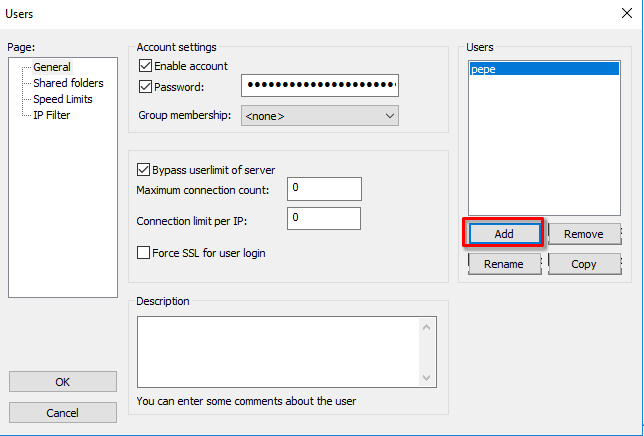
\includegraphics[width=.9\linewidth]{./media/2.png}
\end{center}

Al presionar sobre \emph{add} lo que ocurrirá es que nos aparecerá una ventana solicitando el nombre del nuevo usuario que queremos crear.

Después en la página de \emph{shared folders}, tendremos que presionar en \emph{add} en nuevo para añadir una nueva carpeta. Lo que vamos a hacer es, en disco local (\texttt{C:\textbackslash{}}) vamos a crear una nueva
carpeta que se llame \textbf{Filezilla}, y dentro de la misma, crear una carpeta \textbf{serei} para nuestro nuevo usuario.

\begin{center}
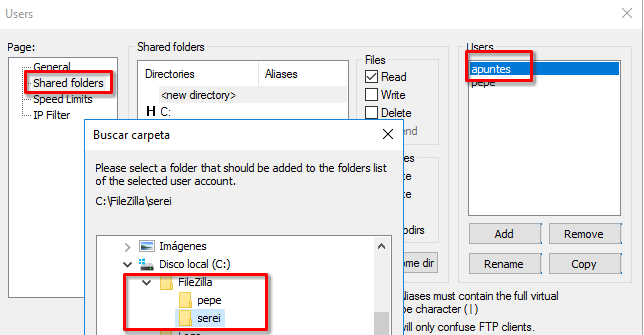
\includegraphics[width=.9\linewidth]{./media/3.png}
\end{center}

Ahora le tendremos que asignar los permisos que deseemos sobre este directorio a este usuario. En mi caso le voy a dar todos, ya que es su propio directorio. Podríamos dejar menos para un
directorio compartido o anónimo. Dados los permisos, tenemos que presionar sobre la opción de \textbf{\emph{Set as home dir}} para que sea considerado su \texttt{\$HOME} y sea donde conecte el usuario por defecto

\begin{center}
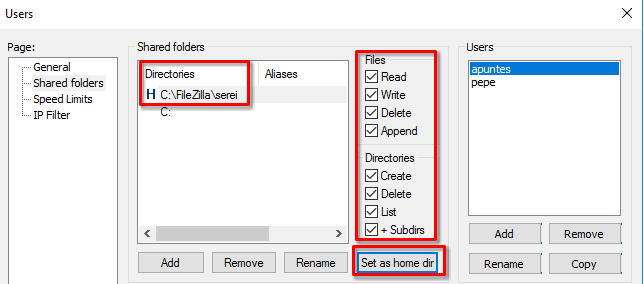
\includegraphics[width=.9\linewidth]{./media/4.png}
\end{center}

\subsubsection{Conexión desde un cliente}
\label{sec:org43fdea0}
Ahora vamos a comprobar si funciona el servidor conectándonos desde un cliente tanto \emph{Windows 10 LTSC} como GNU/Linux.

\begin{enumerate}
\item Conexión desde un cliente \emph{Windows}
\label{sec:org908f80f}
Para conectarnos desde un \emph{Windows 10} cliente lo primero que tendremos que hacer será tener instalado el programa \texttt{Filezilla} cliente en nuestra máquina cliente.

\begin{center}
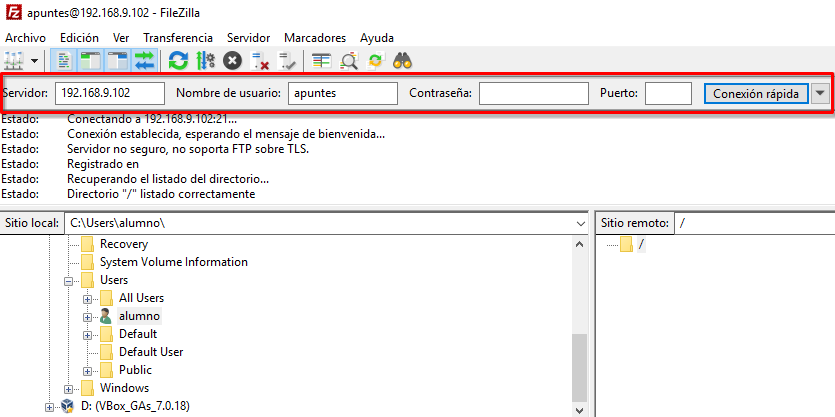
\includegraphics[width=.9\linewidth]{./media/5.png}
\end{center}

\item Conexión desde un cliente GNU/Linux
\label{sec:org5d05857}
Para conectarnos desde un cliente GNU/Linux (en mi caso una máquina Fedora 39), lo que tendremos que hacer será usar la instrucción \texttt{ftp} desde una terminal de la siguiente manera:
\begin{itemize}
\item \texttt{ftp <DIRECCION IP SERVIDOR>}
\end{itemize}

\begin{minted}[,frame=single]{bash}
maka:~/ $ ftp 192.168.9.102                                                                                [15:34:38]
Connected to 192.168.9.102 (192.168.9.102).
220-FileZilla Server 0.9.51 beta
220-written by Tim Kosse (tim.kosse@filezilla-project.org)
220 Please visit https://filezilla-project.org/
Name (192.168.9.102:maka): apuntes
331 Password required for apuntes
Password:
230 Logged on
Remote system type is UNIX.
ftp> 
\end{minted}
\end{enumerate}




\subsubsection{Configuración del servidor}
\label{sec:org8eb50db}
\begin{enumerate}
\item Creación de un grupo
\label{sec:orgd8bbdba}
Ahora vamos a probar a crear un grupo para poder gestionar los usuarios de forma colectiva. El procedimiento es prácticamente igual que crear un usuario, pero presionando sobre el icono que
muestra \textbf{dos personas}.

\begin{center}
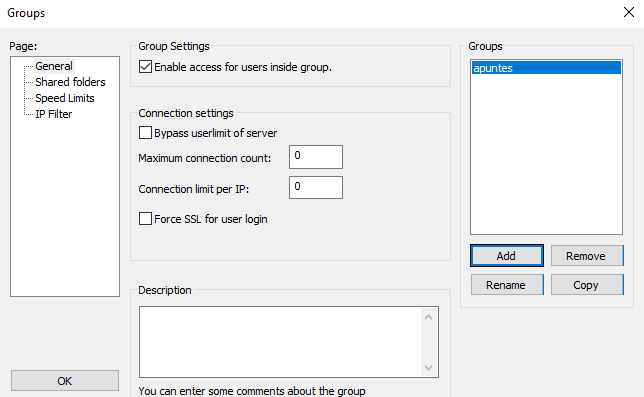
\includegraphics[width=.9\linewidth]{./media/6.png}
\end{center}

También crearemos una carpeta compartida para el grupo, en este caso con una peculiaridad. Después de asignar la carpeta, en este caso la he llamado ASIR, como el grupo, vamos a seleccionar
la opción de \textbf{\emph{Rename}}, y le añadiremos un \texttt{\textbackslash{}u:}. Además pondremos la casilla de \textbf{\emph{autocreate}}. De esta forma le asginamos a cada usuario del grupo que se conecte por FTP una carpeta propia,
y además, no tendremos que crearla nosotros, sino que se creará automáticamente en la primera conexión de cada usuario.

\begin{center}
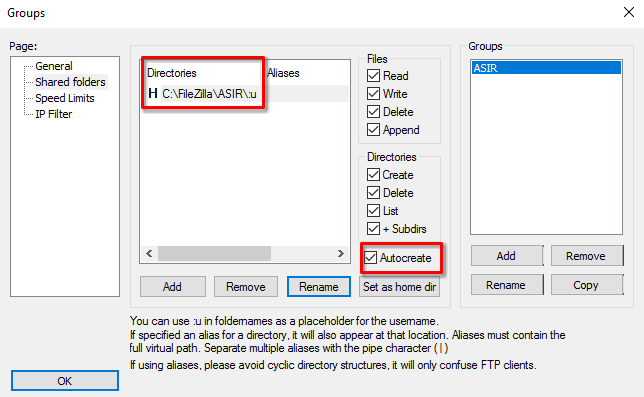
\includegraphics[width=.9\linewidth]{./media/7.png}
\end{center}
\item Limitación de acceso
\label{sec:orgda24acc}
En la pestaña de \textbf{\emph{edit > Settings}} podemos ver en \textbf{\emph{General settings}} dos opciones:
\begin{itemize}
\item \textbf{IP BINDINGS} --> Donde elegimos las direcciones IP por la que tenemos disponible el servidor FTP. Si ponemos un * significará que ofrecemos el servicio por todas las direcciones IP disponibles.
\item \textbf{IP FILTER} --> Para filtrar las IPs que pueden acceder al servidor. Se puede filtrar por IP concreta (sin máscara de subred) o por rangos IP (subredes con máscaras de subred)
\end{itemize}
\end{enumerate}

\subsubsection{Conexión segura por SSL}
\label{sec:org3bb89b1}
Para hacer segura la conexión del servidor, de nuevo en \textbf{\emph{edit > settings}}, ahora en el apartado de \textbf{\emph{FTP over TLS settings}}.

En este caso presionaremos sobre \textbf{\emph{Generate new certificate}} y rellenaremos los campos. En el \emph{common name}, según el cliente FTP que usemos, será necesario poner el nombre que usaremos
en el momento de establecer la conexión.

\begin{center}
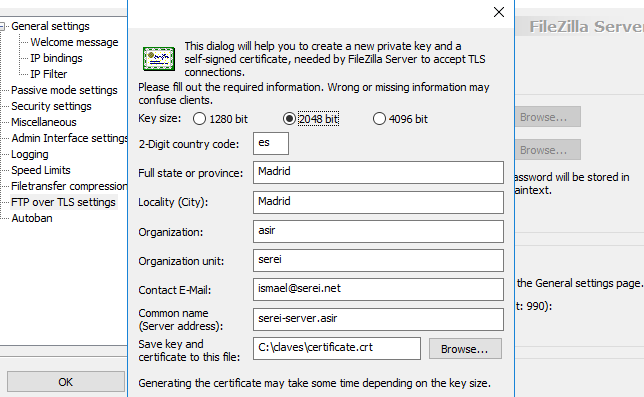
\includegraphics[width=.9\linewidth]{./media/8.png}
\end{center}

Al usar esta creación de certificado se crea solo un fichero \emph{certificate.crt} que contiene tanto el certificado como la clave privada.

\begin{center}
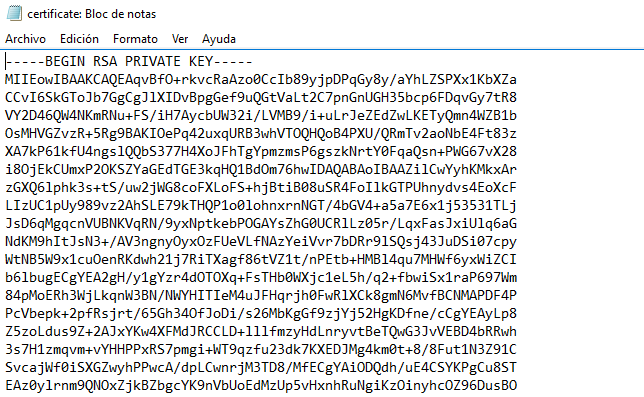
\includegraphics[width=.9\linewidth]{./media/9.png}
\end{center}

Aquí podemos verlo. Será necesario sacar las dos partes a dos ficheros separados, uno \emph{private.key} con la clave privada y otro \emph{certificatePublica.crt} con el certificado.

\begin{center}

\includegraphics[width=.9\linewidth]{./media/10.png}
\end{center}

Y ahora tendremos que indicar en la configuración la ruta de los ficheros.

\begin{center}
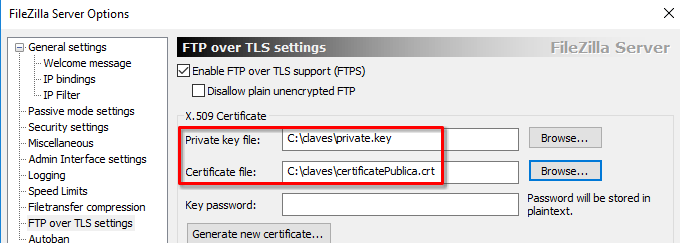
\includegraphics[width=.9\linewidth]{./media/11.png}
\end{center}

Cuando nos conectemos desde un cliente mediante \texttt{FTPS}, como el certificado no está firmado por una entidad verificadora, sino que lo hemos hecho a nivel local de una forma casera, será
necesario cancelar la verificación del certificado. Para ello, una vez hayamos establecido la conexión habrá que escribir lo siguiente:
\begin{itemize}
\item \texttt{set ssl:verify-content no}
\end{itemize}

En caso de querer hacer está configuración de manera permanente lo que tendremos que hacer será modificar el fichero \texttt{/etc/lftp.conf} y poner en el final las siguientes líneas
\begin{minted}[,frame=single]{bash}
set dns:order "inet6 inet"
set ssl:verify-certificate no
\end{minted}

\begin{enumerate}
\item Comprobación de conexión mediante \texttt{FTPD}
\label{sec:org626de4c}
Tendremos que realizar una conexión mediante \texttt{lftp}
\begin{minted}[,frame=single]{bash}
maka:~/ $ lftp -u apuntes ftps://192.168.9.102                                                             [16:38:22]
Password: 
lftp apuntes@192.168.9.102:~>
\end{minted}


\item Comprobación de firma del certificado en una máquina GNU/Linux
\label{sec:orgc51641e}
\begin{itemize}
\item \texttt{openssl x509 -in certificatePublica.crt -noout -fingerprint -[sha256|sha1]}
\end{itemize}
\end{enumerate}

\section{SSH}
\label{sec:org552942f}
\subsection{\texttt{Telnet}}
\label{sec:orge273e5c}
\begin{itemize}
\item El paquete de \texttt{telnet} es \textbf{\texttt{telnetd}}
\end{itemize}
\subsection{Ficheros relevantes}
\label{sec:orgbf63ce2}
\begin{itemize}
\item \texttt{/etc/ssh/ssh\_config}: fichero de configuración de parámetros del cliente
\item \texttt{/etc/ssh/sshd\_config}: fichero de configuración de parámetros del servidor
\item \texttt{\$HOME/.ssh/authorized\_keys}: fichero que contiene las claves públicas de los hosts autorizados a conectarse por autenticación de clave pública
\item \texttt{\$HOME/.ssh/known\_hosts}: guarda las conexiones que se han realizado a servidores \texttt{ssh} una vez aceptadas las \emph{fingerprints}
\item \texttt{\$HOME/.ssh/config}: nos permite configurar ciertos parámetros de los que se definene en el fichero \texttt{/etc/ssh/ssh\_config} pero de manera individual para el usuarios que lo usa y para la
conexión concreta especificada
\end{itemize}
\subsection{Instalación del servidor \texttt{openssh}}
\label{sec:orga1e2789}
Para instalar un servidor \texttt{ssh} lo que tendremos que hacer será hacer uso de la instrucción:
\begin{itemize}
\item \texttt{sudo apt-get install openssh-server}
\end{itemize}


En caso de querer instalar un cliente \texttt{ssh} tendremos que hacer uso de la instrucción:
\begin{itemize}
\item \texttt{sudo apt-get install openssh-client}
\end{itemize}


Luego podremos establecer una conexión al servidor desde un cliente ejecutando la instrucción
\begin{itemize}
\item \texttt{ssh nombreUsuario@DireccionIPMaquin}
\end{itemize}
\begin{minted}[,frame=single]{bash}
maka@ubuntu3:~$ ssh maka@172.20.10.5
The authenticity of host '172.20.10.5 (172.20.10.5)' can't be established.
ECDSA key fingerprint is e6:cf:d5:13:d4:cf:7e:b7:9a:01:6c:86:c6:23:6f:75.
Are you sure you want to continue connecting (yes/no)? yes
Warning: Permanently added '172.20.10.5' (ECDSA) to the list of known hosts.
maka@172.20.10.5's password: 
Welcome to Ubuntu 14.04.6 LTS (GNU/Linux 4.4.0-142-generic x86_64)

 * Documentation:  https://help.ubuntu.com/

Your Hardware Enablement Stack (HWE) is supported until April 2019.

The programs included with the Ubuntu system are free software;
the exact distribution terms for each program are described in the
individual files in /usr/share/doc/*/copyright.

Ubuntu comes with ABSOLUTELY NO WARRANTY, to the extent permitted by
applicable law.

maka@ubuntu2:~$
\end{minted}
\subsection{Ver la dirección en \texttt{known\_hosts} en vez de el \texttt{hash}}
\label{sec:org79900f9}
Ahora lo que haremos será hacer configuraciones para que en vez de ver un \texttt{hash} cuando miremos el fichero \texttt{\$HOME/.ssh/known\_hosts} veámos la dirección IP que se ha conectado a nuestro servidor.

Primero antes de hacer nada lo que haremos será mirar en la máquina servidor el fichero \texttt{\$HOME/.ssh/known\_hosts} para ver si tenemos algún registro
\begin{minted}[,frame=single]{bash}
maka@ubuntu2:~/.ssh$ cat known_hosts 
|1|VJm5fgA1jJBxCHzMjP+651QexPY=|SsSzyK9hTHUzxSpDMeWhlGgznuk= ecdsa-sha2-nistp256 AAAAE2VjZHNhLXNoYTItbmlzdHAyNTYAAAAIbmlzdHAyNTYAAABBBNfC3VlFMn7jXU61ITQBxbRBRTv8E5Z/hNokk5W12Hgac
7CB2ErfSGex08oqOJQtLUXfLYjruHe8h8XBy7UKVJg=
\end{minted}

Lo que se puede apreciar arriba es la entrada que tenemos en el fichero \texttt{\$HOME/.ssh/known\_hosts} de nuestra máquina servidor después de haber realizado un \texttt{ssh} desde nuestra máquina cliente.

Para ver la dirección IP que se ha conectado a nosotros en vez de ese \texttt{hash} lo que tendremos que hacer será, en nuestra máquina servidor, modificar el fichero \texttt{/etc/ssh/ssh\_config} en la
línea que contenga \texttt{HashKnownHosts} de tal manera que su valor sea \texttt{no}.
\begin{minted}[,frame=single]{bash}
#   RekeyLimit 1G 1h
    SendEnv LANG LC_*
    HashKnownHosts no
\end{minted}

NO FUNCIONA
\subsection{Eliminar error intento ataque Ddos}
\label{sec:orgbe324f3}
Muchas veces vamos a tener que eliminar entradas de nuestro fichero \texttt{known\_hosts} para que al cliente le vuelva a aparecer el mensaje del \emph{fingerprint}, para hacer esto tendremos que usar
la instrucción:
\begin{itemize}
\item \texttt{ssh-keygen -f \$HOME/.ssh/known\_hosts -R DIRECCIONIPCLIENTE}
\end{itemize}
\subsection{Conexión por clave pública}
\label{sec:org0f8f338}
Lo primero que tendremos que hacer será generar un par de claves pública-privada en el cliente.

Para generar estás claves tendremos que hacer uso de la instrucción \texttt{ssh-keygen} de la siguiente manera:
\begin{itemize}
\item \texttt{ssh-keygen -t rsa}
\end{itemize}
\begin{minted}[,frame=single]{bash}
maka@ubuntu201:~$ ssh-keygen -t rsa
Generating public/private rsa key pair.
Enter file in which to save the key (/home/maka/.ssh/id_rsa): 
Enter passphrase (empty for no passphrase): 
Enter same passphrase again: 
Your identification has been saved in /home/maka/.ssh/id_rsa.
Your public key has been saved in /home/maka/.ssh/id_rsa.pub.
The key fingerprint is:
30:c2:99:66:79:3b:1a:93:d0:aa:13:67:65:7d:47:20 maka@ubuntu201
The key's randomart image is:
+--[ RSA 2048]----+
|      E ...      |
|   o = . .       |
|  . % = . .      |
|   B + = .       |
|. + + o S        |
| =   + .         |
|o   .            |
| .               |
|                 |
+-----------------+
\end{minted}

Las claves se almacenarán en \texttt{\$HOME/.ssh/}
\begin{minted}[,frame=single]{bash}
maka@ubuntu201:~$ ls -la .ssh/
total 20
drwx------  2 maka maka 4096 feb 18 18:35 .
drwxr-xr-x 19 maka maka 4096 feb 18 18:32 ..
-rw-------  1 maka maka 1679 feb 18 18:35 id_rsa
-rw-r--r--  1 maka maka  396 feb 18 18:35 id_rsa.pub
-rw-r--r--  1 maka maka  444 dic  9 09:39 known_hosts
\end{minted}

Luego de haber creado las claves lo que tendremos que hacer será enviar la \textbf{clave pública} al servidor, en mi caso lo haré mediante la instrucción \texttt{scp}
\begin{itemize}
\item \texttt{maka@ubuntu201:\textasciitilde{}\$ scp .ssh/id\_rsa.pub ana@172.20.10.5:/home/ana/}
\end{itemize}

Una vez tengamos la clave pública del cliente en el servidor lo que tendremos que hacer será añadir la clave al fichero \texttt{\$HOME/.ssh/authorized\_keys}


\begin{alertblock}{AVISO}
Puede que el fichero authorized keys no exista. En ese caso lo que haremos sera renombrar la clave pública con el nombre de authorized key
\end{alertblock}

\begin{minted}[,frame=single]{bash}
root@ubuntu2:/etc/ssh# cd /home/ana/.ssh/
root@ubuntu2:/home/ana/.ssh# ls -la
total 12
drwx------ 2 ana ana 4096 feb 18 18:55 .
drwxr-xr-x 4 ana ana 4096 feb 18 18:41 ..
-rw-r--r-- 1 ana ana  396 feb 18 18:38 authorized_keys
-rw-r--r-- 1 ana ana    0 feb 18 18:26 known_hosts
\end{minted}

Ahora tendríamos que poder acceder desde la máquina cliente a la máquina servidor sin tener que escribir ningún tipo de \emph{password}
\begin{minted}[,frame=single]{bash}
maka@ubuntu201:~$ ssh ana@172.20.10.5
Welcome to Ubuntu 14.04.6 LTS (GNU/Linux 4.4.0-142-generic x86_64)

 * Documentation:  https://help.ubuntu.com/

New release '16.04.7 LTS' available.
Run 'do-release-upgrade' to upgrade to it.

Your Hardware Enablement Stack (HWE) is supported until April 2019.
Last login: Tue Feb 18 18:42:54 2025 from 172.20.10.2
ana@ubuntu2:~$ 
\end{minted}

Con la opción \texttt{-v} de la instrucción \texttt{ssh} podríamos ver el proceso en el cuál se leen las claves. La opción que nos daría la mejor información de lo que está pasando sería
\begin{itemize}
\item \texttt{debug1: Offering RSA public key: /home/maka/.ssh/id\_rsa}
\end{itemize}

En caso de tener más de una clave en nuestro cliente tendríamos que usar la opción \texttt{-i} de la instrucción \texttt{ssh} de la siguiente manera:
\begin{itemize}
\item \texttt{ssh -i <{}<{}NOMBRE-CLAVE-PRIVADA>{}>{} usuario@destino}
\end{itemize}
\subsubsection{Configuración del servidor}
\label{sec:orgb79d404}
Podemos habilitar o deshabilitar la conexión mediante claves público-privada con la opción \texttt{PubKeyAuthentication} en el fichero \texttt{/etc/ssh/sshd\_config}
\subsection{Directorio \texttt{\$HOME/.ssh/}}
\label{sec:org0c4bbe4}
Es un directorio el cuál se crea solo en la \texttt{\$HOME} del usuario con el que estés conectando. Para añadir ciertos parámetros de configuración, debemos crear un fichero llamado \texttt{config} y ahí
podemos poner los parámetros que queramos.
\begin{minted}[,frame=single]{bash}
Host 172.20.10.5-rsa
    Hostname 172.20.10.5
    HostKeyAlgorithms ssh-rsa
    ForwardX11 yes
    CheckHostIp no
    HostKeyAlias 172.20.10.5-rsa
    Port 2222
    User ana
\end{minted}
\begin{itemize}
\item \texttt{Hostname 172.20.10.5}: Dirección IP a la que se conecta
\item \texttt{HostKeyAlgorithms ssh-rsa}: El cliente solo usará el algoritmo \texttt{ssh-rsa} para autenticarse con el servidor
\item \texttt{ForwardX11 yes}: Habilita el reenvío de las X11, permitiendo ejecutar aplicaciones gráficas en el servidor viéndolas en el cliente
\item \texttt{CheckHostIp no}: Evita que \texttt{ssh} verifique si la IP del servidor ha cambiado
\item \texttt{HostKeyAlias 172.20.10.5-rsa}: usa 172.20.10.5-rsa como alías para la clave del host en \texttt{\textasciitilde{}/.ssh/known\_hosts}
\item \texttt{Port 2222}: En lugar del puerto estándar (22), usará el puerto 2222
\item \texttt{User ana}: Especifica el usuario con el hará \emph{login} en el servidor
\end{itemize}
\subsection{Algoritmo de cifrado}
\label{sec:orgfb9c5a1}
El algoritmo por defecto es \texttt{ecdsa-sha2-nistp256}, pero lo podemos modificar estableciendo la conexión de la siguiente manera:
\begin{itemize}
\item \texttt{ssh -o HostKeyAlgorithms=ssh-rsa ana@172.20.10.5}
\end{itemize}

Si no eliminamos el contenido del fichero \texttt{\$HOME/,ssh/known\_hosts} nos aparecerá el siguiente error
\begin{minted}[,frame=single]{bash}
@@@@@@@@@@@@@@@@@@@@@@@@@@@@@@@@@@@@@@@@@@@@@@@@@@@@@@@@@@@
@    WARNING: REMOTE HOST IDENTIFICATION HAS CHANGED!     @
@@@@@@@@@@@@@@@@@@@@@@@@@@@@@@@@@@@@@@@@@@@@@@@@@@@@@@@@@@@
IT IS POSSIBLE THAT SOMEONE IS DOING SOMETHING NASTY!
Someone could be eavesdropping on you right now (man-in-the-middle attack)!
It is also possible that a host key has just been changed.
The fingerprint for the RSA key sent by the remote host is
ec:ed:1e:48:f1:8d:22:4e:e2:dc:58:e1:c6:b0:f7:d0.
Please contact your system administrator.
Add correct host key in /home/maka/.ssh/known_hosts to get rid of this message.
Offending ECDSA key in /home/maka/.ssh/known_hosts:3
  remove with: ssh-keygen -f "/home/maka/.ssh/known_hosts" -R 172.20.10.5
RSA host key for 172.20.10.5 has changed and you have requested strict checking.
Host key verification failed.
\end{minted}

Lo único que tendremos que hacer será ejecutar la instrucción \texttt{echo "" > known\_hosts} para eliminar el contenido del fichero y ya nos podremos conectar y encima sin contraseña porque tenemos
la clave pública en el servidor
\begin{minted}[,frame=single]{bash}
maka@ubuntu201:~/.ssh$ echo "" > known_hosts 
maka@ubuntu201:~/.ssh$ ssh -o HostKeyAlgorithms=ssh-rsa ana@172.20.10.5
The authenticity of host '172.20.10.5 (172.20.10.5)' can't be established.
RSA key fingerprint is ec:ed:1e:48:f1:8d:22:4e:e2:dc:58:e1:c6:b0:f7:d0.
Are you sure you want to continue connecting (yes/no)? yes
Warning: Permanently added '172.20.10.5' (RSA) to the list of known hosts.
Welcome to Ubuntu 14.04.6 LTS (GNU/Linux 4.4.0-142-generic x86_64)

 * Documentation:  https://help.ubuntu.com/

New release '16.04.7 LTS' available.
Run 'do-release-upgrade' to upgrade to it.

Your Hardware Enablement Stack (HWE) is supported until April 2019.
Last login: Tue Feb 18 18:57:13 2025 from 172.20.10.2
\end{minted}
\subsection{\texttt{SSH-Agent}}
\label{sec:orge3c2828}
Es un programa que gestiona las claves privadas \texttt{ssh} en segundo plano, evitando que tengas que ingresar la contraseña de tu clave privada cada vez que te conectas a un servidor, incluso evita
tener que ingresar la clave de paso.

Vamos a generar una clave que tenga frase de paso para comprobar que esto es cierto.

Para generar la clave de paso tendremos que hacer uso de la instrucción \texttt{ssh-keygen -t rsa}
\begin{minted}[,frame=single]{bash}
maka@ubuntu201:~$ ssh-keygen -t rsa
Generating public/private rsa key pair.
Enter file in which to save the key (/home/maka/.ssh/id_rsa): id_rsa_frase
Enter passphrase (empty for no passphrase): 
Enter same passphrase again: 
Your identification has been saved in id_rsa_frase.
Your public key has been saved in id_rsa_frase.pub.
The key fingerprint is:
6c:33:c5:1d:58:28:32:17:3a:c1:30:8c:48:62:dc:07 maka@ubuntu201
The key's randomart image is:
+--[ RSA 2048]----+
|++.E+o. .. +o    |
|+....o+oo.o. .   |
|    . o+ .o .    |
|       o .       |
|        S        |
|       . o       |
|                 |
|                 |
|                 |
+-----------------+
\end{minted}

Ahora tendremos que ejecutar la instrucción \texttt{ssh-agent} y añadiremos la nueva frase de paso
\begin{minted}[,frame=single]{bash}
maka@ubuntu201:~$ ssh-agent 
SSH_AUTH_SOCK=/tmp/ssh-Fh3MJaBVg9pL/agent.4470; export SSH_AUTH_SOCK;
SSH_AGENT_PID=4471; export SSH_AGENT_PID;
echo Agent pid 4471;
maka@ubuntu201:~$ ssh-add id_rsa_frase
Enter passphrase for id_rsa_frase: 
Identity added: id_rsa_frase (id_rsa_frase)
\end{minted}

Con la instrucción \texttt{ssh-add -l} listamos las frases de paso que tengamos
\begin{minted}[,frame=single]{bash}
maka@ubuntu201:~$ ssh-add -l
2048 6c:33:c5:1d:58:28:32:17:3a:c1:30:8c:48:62:dc:07 id_rsa_frase (RSA)
2048 30:c2:99:66:79:3b:1a:93:d0:aa:13:67:65:7d:47:20 maka@ubuntu201 (RSA)
\end{minted}

Ahora lo que tendremos que hacer será enviar la clave pública al servidor, en mi caso seguiré usando la instrucción \texttt{scp}
\begin{itemize}
\item \texttt{maka@ubuntu201:\textasciitilde{}\$ scp id\_rsa\_frase.pub ana@172.20.10.5:/home/ana}
\end{itemize}

Una vez tengamos la clave pública nueva en la máquina servidor lo que haremos será ejecutar una instrucción la cuál lee el contenido del fichero de la clave pública y lo añade al fichero de
\texttt{\$HOME/.ssh/authorized\_keys}
\begin{itemize}
\item \texttt{cat id\_rsa\_frase.pub >{}>{} .ssh/authorized\_keys}
\end{itemize}

Y ya nos podríamos conectar usando la opcíon \texttt{i} con esa frase de paso
\begin{minted}[,frame=single]{bash}
maka@ubuntu201:~$ ssh -i id_rsa_frase ana@172.20.10.5
Welcome to Ubuntu 14.04.6 LTS (GNU/Linux 4.4.0-142-generic x86_64)

 * Documentation:  https://help.ubuntu.com/

New release '16.04.7 LTS' available.
Run 'do-release-upgrade' to upgrade to it.

Your Hardware Enablement Stack (HWE) is supported until April 2019.
Last login: Tue Feb 18 19:19:15 2025 from 172.20.10.2
ana@ubuntu2:~$ 
\end{minted}
\subsection{Windows: \texttt{ssh}, claves y \texttt{ssh-agent}}
\label{sec:org609b1a8}
Para instalar el servidor OpenSSH en una máquina Windows 10 la ruta a seguir es:
\begin{enumerate}
\item Ajustes
\item Aplicaciones
\item Aplicaciones y características
\item Administrar funciones opcionales
\item Agregar una característica
\end{enumerate}

El \texttt{ssh-agent} se habilita en \textbf{Servicios} > \emph{OpenSSH Authentication Agent}. Lo pondremos en automático

\begin{center}
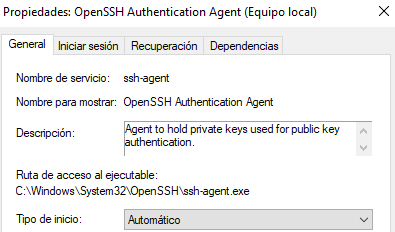
\includegraphics[width=.9\linewidth]{./media/ssh-agent-win.png}
\end{center}

Para generar un par de claves público-privada en Windows se hará con la misma instrucción usada en GNU/Linux desde el \texttt{CMD}

\begin{center}
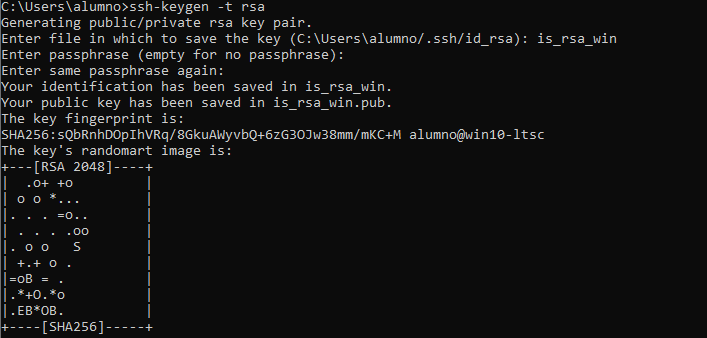
\includegraphics[width=.9\linewidth]{./media/ssh-keygen-win.png}
\end{center}

Luego le daremos la clave pública al servidor mediante la instrucción \texttt{scp}

Luego en el servidor lo que haremos será añadir el contenido de la clave pública al fichero \texttt{/.ssh/authorized\_key}

Ya nos podremos conectar sin ningún tipo de problema.

\subsubsection{Putty}
\label{sec:org5356944}
Lo primero que haremos será instalar el \emph{software} putty

Una vez instalado el \emph{software} lo que haremos será abrir el programa \textbf{PuttyGen} para crear un par de claves

\begin{center}
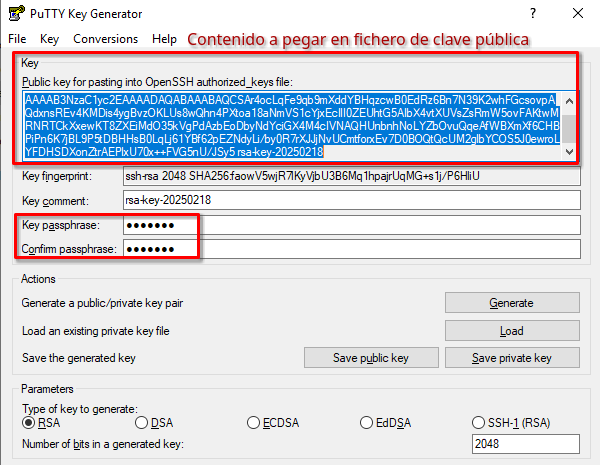
\includegraphics[width=.9\linewidth]{./media/win-puttygen.png}
\end{center}

Luego de tener algo parecido a lo que se puede ver en la imagen de arriba lo que haremos será:
\begin{enumerate}
\item Añadir la clave de paso
\item Copiar el texto que aparece en rojo porque será el contenido de la clave pública
\item Presionar los botónes de \emph{save public key \& save private key}
\end{enumerate}

Después de esto ya podremos realizar el procedimiento ya conocido de:
\begin{enumerate}
\item Enviar la clave pública al servidor mediante \texttt{scp}
\item Añadir en el servidor la clave pública al fichero \texttt{.ssh/authorized\_keys}
\end{enumerate}

En este caso probaré a conectarme a la máquina servidor desde el \emph{software} Putty y no desde el \texttt{cmd}.

\begin{center}
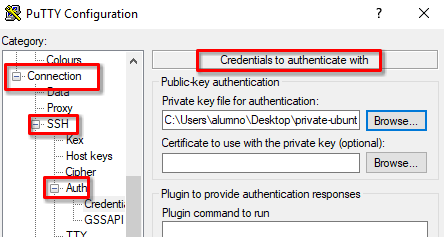
\includegraphics[width=.9\linewidth]{./media/putty-connect.png}
\end{center}

\begin{center}
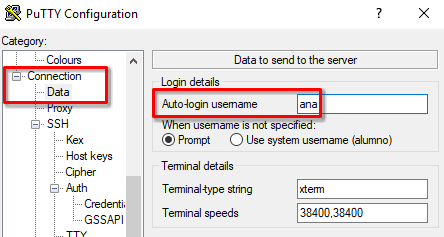
\includegraphics[width=.9\linewidth]{./media/putty-connect-2.png}
\end{center}

\begin{center}
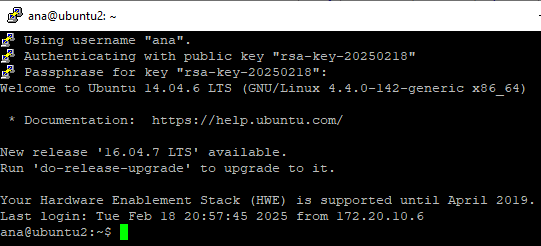
\includegraphics[width=.9\linewidth]{./media/putty-connect-3.png}
\end{center}

Se puede apreciar en la última imagen de arriba que aún nos está pidiendo la frase de paso. Para evitar esto lo que tendremos que hacer será abrir el programa \textbf{Pageant} y añadir el agente.

Cuando presionemos sobre \textbf{Pageant} en el buscador de \emph{windows} no ocurrirá nada especial, pero "aparecerá" lo siguiente

\begin{center}
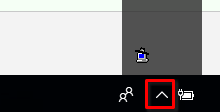
\includegraphics[width=.9\linewidth]{./media/pageant-1.png}
\end{center}

Lo que haremos será hacer clic derecho sobre ese icono > añadir clave y añadiremos nuestra clave privada.

Luego en la configuración de Putty lo que haremos será en conexión > ssh > auth, marcar la casilla de autenticarse usando pageant

\begin{center}
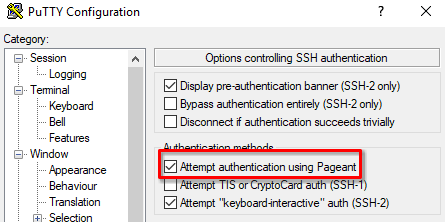
\includegraphics[width=.9\linewidth]{./media/pageant-2.png}
\end{center}

\begin{center}
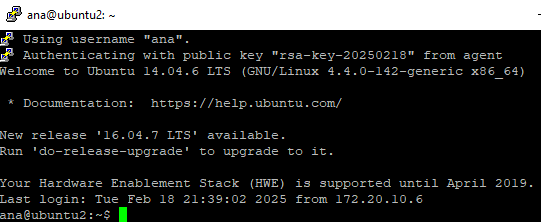
\includegraphics[width=.9\linewidth]{./media/pageant-3.png}
\end{center}

Como se puede apreciar ya no se nos pide la frase de paso para acceder al usuario ana.

\subsubsection{MobaXterm}
\label{sec:org57d8fdc}
Para generar un par de claves público-privadas en mobaxterm lo que hay que hacer es ir a \emph{tools} > MobaKeyGen

La interfaz es casi igual a la de putty por lo que habrá que hacer clic en \textbf{generar claves} y mover el ratón.

En este caso no vamos a crear ningún par de claver pero lo que si que vamos a hacer es realizar una conexión usando este programa.

\begin{center}
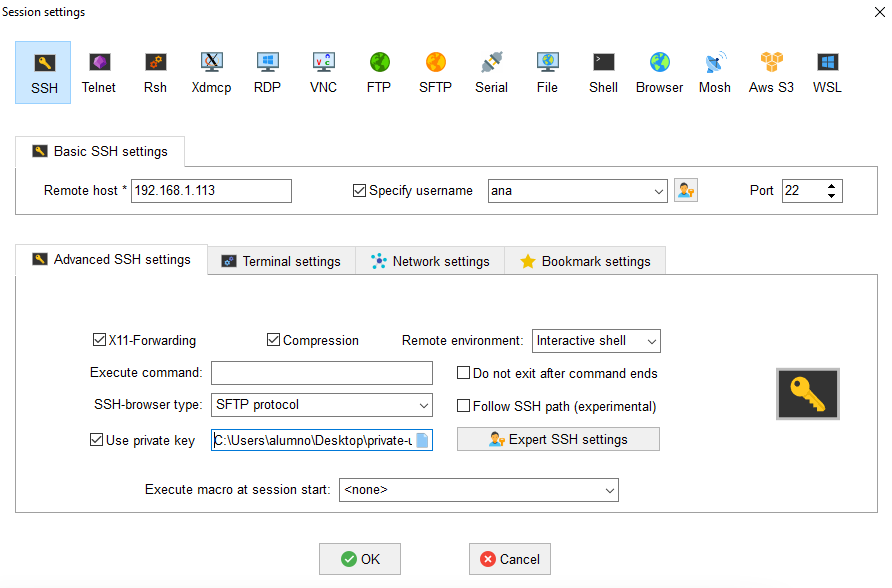
\includegraphics[width=.9\linewidth]{./media/mobaxterm.png}
\end{center}

\begin{center}
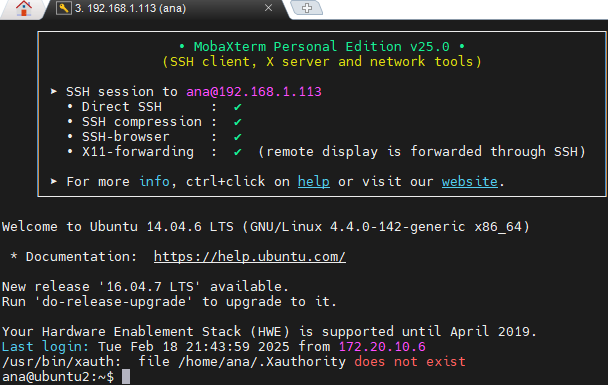
\includegraphics[width=.9\linewidth]{./media/mobaxterm-2.png}
\end{center}

\begin{alertblock}{AVISO}
Hay que tener iniciado el Pageant para que funcione
\end{alertblock}

Con MobaXterm también podemos conectarnos de una manera gráfica vamos al apartado de \textbf{\emph{Session} > SFTP}

\begin{center}
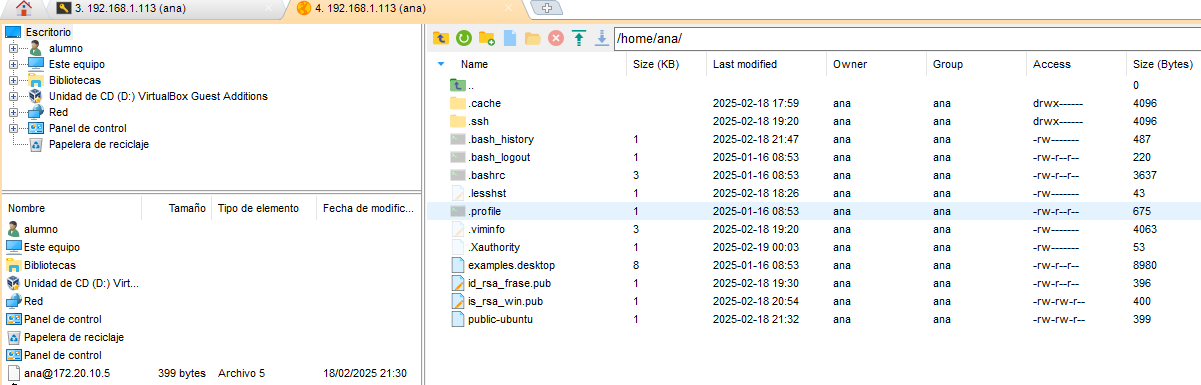
\includegraphics[width=.9\linewidth]{./media/mobaxterm-3.png}
\end{center}
\subsection{Cluster \texttt{ssh}}
\label{sec:orgcd7c026}
Para instalar \texttt{cssh} habrá que ejecutar la instrucción:
\begin{itemize}
\item \texttt{sudo apt-get install clusterssh}
\end{itemize}

Ahora ejecutamos el comando \texttt{cssh} para crear el directorio y sus ficheros de configuración.

\begin{center}
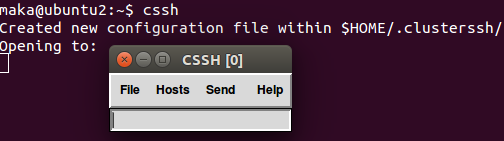
\includegraphics[width=.9\linewidth]{./media/cssh-1.png}
\end{center}

ahora básicamente podremos conectarnos a varias máquinas a la vez, en mi caso me conectaré a otras dos máquinas Ubuntu

\begin{center}
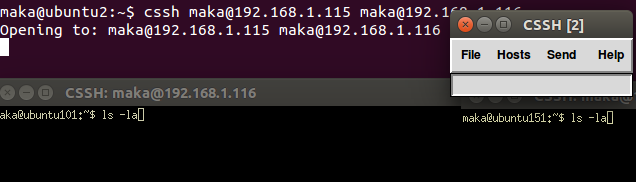
\includegraphics[width=.9\linewidth]{./media/cssh-2.png}
\end{center}

Como se puede ver en la imagen de arriba se me han abierto 3 ventanas, 2 más grandes y una pequeña, las dos grandes corresponden a los equipos que estamos conectados y la pequeña es para que
escribamos los comandos que se escribiran al mismo tiempo en las dos ventanas grandes y cuando presionemos la tecla \texttt{ENTER} se ejecutará el comando en las dos ventanas grandes.

Si las máquinas tuvieran el mismo usuario podríamos usar el siguiente comando:
\begin{itemize}
\item \texttt{cssh -l maka <ip> <ip> <ip>}
\end{itemize}

\subsubsection{{\bfseries\sffamily TODO} Clusters}
\label{sec:org200e192}
Para no tener que estar escribiendo cada vez que queramos conectarnos todas la IPs, podemos crear un grupo de clústers para conectarnos directamente a todos los que estén en ese grupo.

Para ello creamos el fichero en \texttt{\$HOME/maka/.clusterss/clusters}

NO SE SABE


\subsubsection{{\bfseries\sffamily TODO} \emph{Tags}}
\label{sec:orgd3830b6}
En justo lo inverso a cluster.

Crearemos el fichero en \texttt{\$HOME/.clusterssh/tags}
\subsection{Entorno gráfico}
\label{sec:org88ce837}
\subsubsection{GNU/Linux}
\label{sec:orgbc3ad85}
Para poder usar \texttt{ssh} con entorno gráfico, tenemos que habilitarlo en el servidor.

Tendremos que modificar el fichero \texttt{/etc/ssh/sshd\_config} en la línea que contenga \texttt{X11Forwarding yes}
\begin{minted}[,frame=single]{bash}
X11Forwarding yes
X11DisplayOffset 10
PrintMotd no
PrintLastLog yes
TCPKeepAlive yes
#UseLogin no
\end{minted}

Ahora para conectarnos tendremos que usar el parámetro \texttt{-X} o también lo podemos hacer permanente modificando el fichero \texttt{/etc/ssh/ssh\_config}
\begin{minted}[,frame=single]{bash}
Host *
#   ForwardAgent no
    ForwardX11 yes
\end{minted}

Con esto ya podremos conectarnos y ejecutar comandos de forma gráfica
\begin{center}
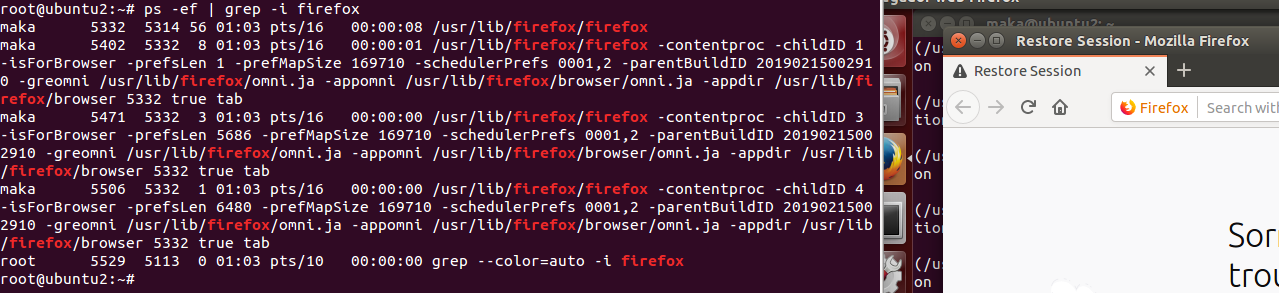
\includegraphics[width=.9\linewidth]{./media/x11-1.png}
\end{center}
\subsubsection{\emph{Microsoft Windows}}
\label{sec:orga5e9139}
En este caso usaremos el programa MobaXterm.

\begin{center}
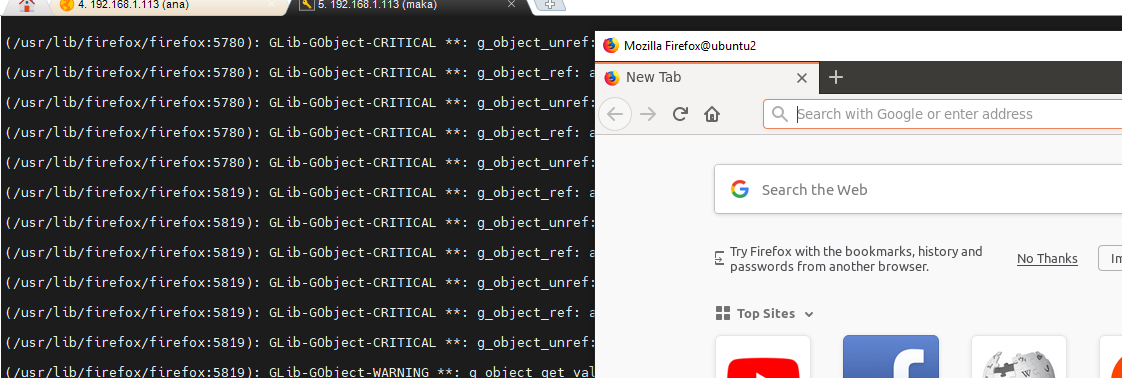
\includegraphics[width=.9\linewidth]{./media/x11-2.png}
\end{center}
\subsection{Tunelización}
\label{sec:orge9bb9f7}
La instrucción a usar sería la siguiente:
\begin{itemize}
\item \texttt{ssh -g -L [interfaz]:[puertoLocal]:[direcciónDelServicio]:[puertoServicio] [conexionSshPuente]}
\end{itemize}

Explicación:
\begin{itemize}
\item \texttt{-g}: \emph{gateway ports}, permite que otros equipos de la red accedan a nuestro puerto de reenvío. Es decir, que puedan acceder a \url{http://NUESTRAIP:NUESTROPUERTO}. Si se usa * como interfaz de
escucha, no sería necesarío especificar este parámetro
\item \texttt{-L}: \emph{local port forwarding}, redirigir el tráfico de un puerto local a otro destino a través de \texttt{ssh}
\item \texttt{[interfazLocal]}: interfaz de red local por la que queremos ofrecer el servicio de la conexión
\item \texttt{[puertoLocal]}: puerto de la máquina local, es decir, la máquina desde la que se ejecuta el comando, por la que queremos que se acceda al servicio accedido
\item \texttt{[direcciónServicio]}: dirección de red, ya sea IP o nombre de la máquina en la que se está sirviendo el servicio y al que queremos acceder
\item \texttt{[puertoServicio]}: puerto por el que se está sirviendo el servicio en la máquina a la que queremos acceder
\item \texttt{[conexionSSHPuente]}: dirección de la máquina puente a través de la cuál queremos acceder a la máquina que contiene el servicio al que queremos acceder
\end{itemize}


\subsubsection{Primer ejemplo}
\label{sec:orgfbdc165}
Tenemos un servidor \texttt{apache2} y otro servidor con \texttt{ssh} además de un cliente, lo que vamos a hacer es pasar al \texttt{apache} del servidor 2 mediante el servidor 1 ya que el servidor 2 no está en
nuestra red.

\begin{center}
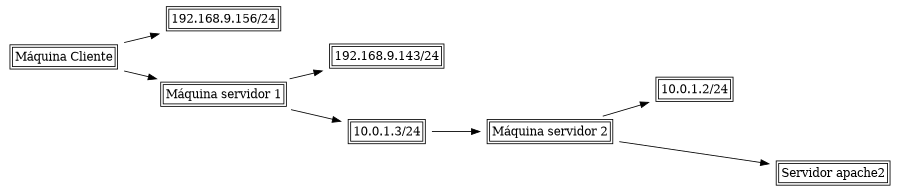
\includegraphics[width=.9\linewidth]{./esquema-ejemplo-uno_diagram.png}
\end{center}

En el cliente ejecutaremos la siguiente instrucción:
\begin{itemize}
\item \texttt{ssh -L 8080:10.1.1.3 maka@192.168.9.143}
\end{itemize}

\begin{center}
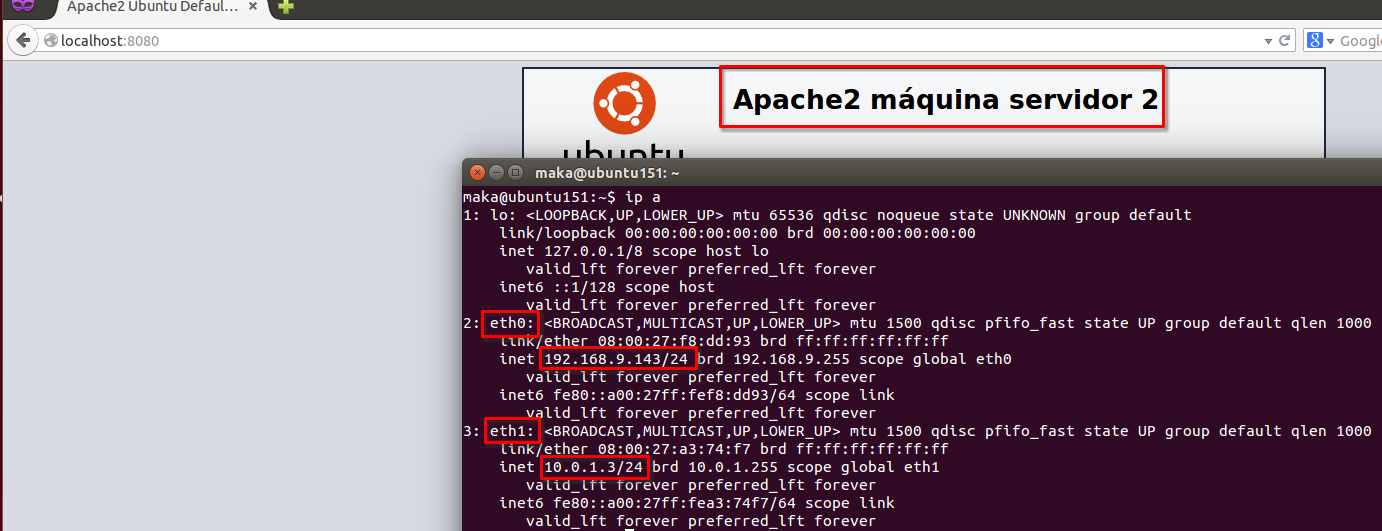
\includegraphics[width=.9\linewidth]{./media/puertos-l.png}
\end{center}

Además si usamos el mismo comando pero con el parámetro \texttt{-g} podremos ver el \texttt{apache} a través de mi máquina real poniendo la IP de la máquina cliente

\begin{center}
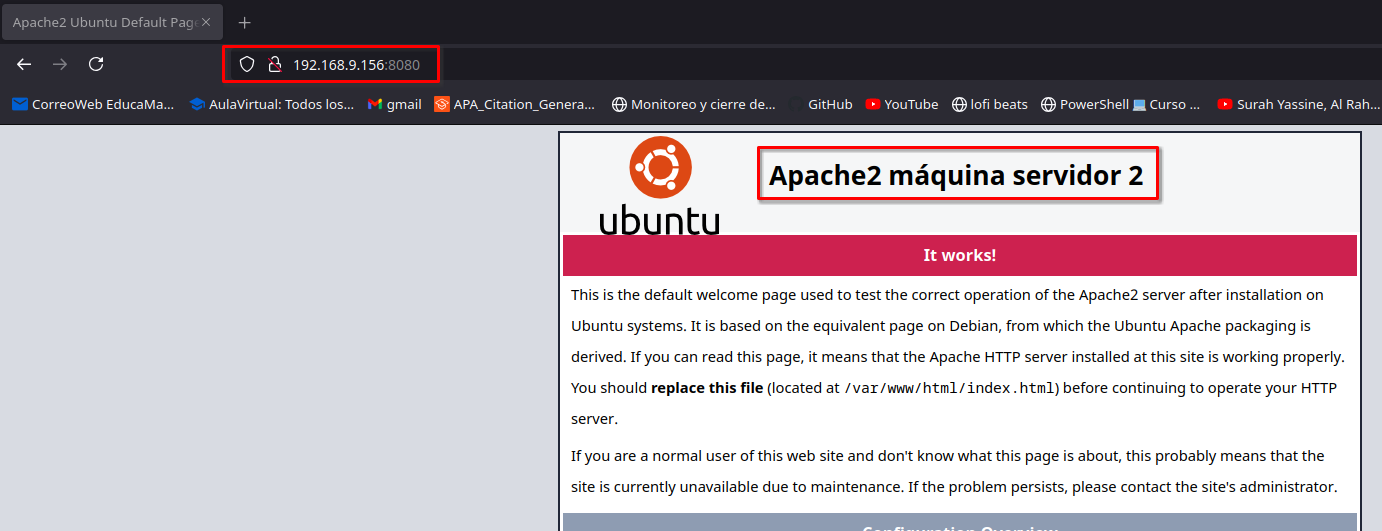
\includegraphics[width=.9\linewidth]{./media/puertos-g.png}
\end{center}

\subsubsection{Túnel remoto}
\label{sec:orgac5e646}
Es igual que antes pero poniendo la opción \texttt{-R}, de esta forma estaríamos sirviendolo en la máquina que estamos usando de "puente"
\begin{itemize}
\item \texttt{ssh -R localhost:8080:10.0.1.2:80 maka@192.168.1.143}
\end{itemize}


Con este comando estamos sirviendo el contenido de la página pero en vez de en mi máquina cliente que ejecuta el comando del servidor
\subsection{Escritorio remoto}
\label{sec:orgc6d9146}
\subsubsection{RDP}
\label{sec:org9f867bc}
Para activar RDP en \emph{windows} seguiremos la siguiente ruta:
\begin{enumerate}
\item Panel de control
\item Sistema de seguridad
\item Sistema
\item Configuración de acceso remoto
\end{enumerate}

\begin{center}
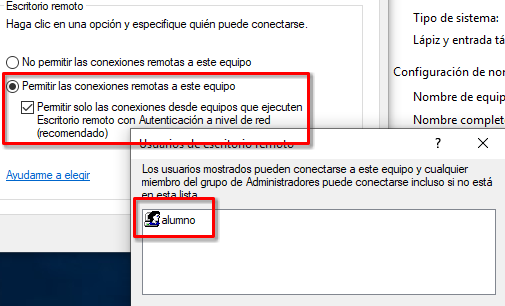
\includegraphics[width=.9\linewidth]{./media/rdp-1.png}
\end{center}

Ahora nos podremos conectar desde otro Windows o GNU/Linux

\begin{center}
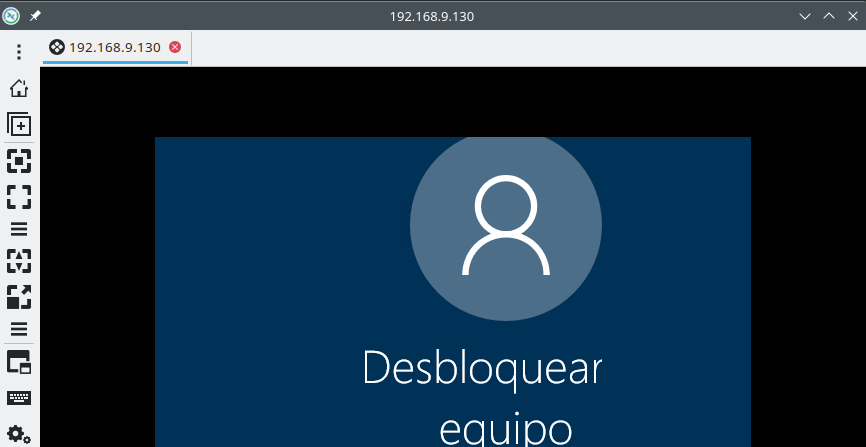
\includegraphics[width=.9\linewidth]{./media/rdp-2.png}
\end{center}

Desde otro S.O Windows podremos conectarnos también a través del cliente nativo o un programa como por ejemplo MobaXterm.
\subsubsection{VNC}
\label{sec:orgd5bef28}
Desde linux o \emph{windows} habrá que instalar un \emph{software} como por ejemplo TightVNC o TigerVNC para tener el servidor y así poder conectarnos.

\section{Servicio web, \texttt{apache2}}
\label{sec:org68e17ad}
\subsection{Instalación}
\label{sec:org7ae091d}
Para instalar el servicio web \texttt{apache2} tendremos que instalar lo siguiente:
\begin{itemize}
\item \texttt{sudo apt-get install apache2}
\item \texttt{sudo apt-get install libapache2-mod-php5}
\item \texttt{sudo apt-get install apache2-utils}
\item \texttt{sudo apt-get install mysql-server mysql-client mysql-common}
\item \texttt{sudo apt-get install phpmyadmin}
\end{itemize}
\subsection{Apuntes teóricos}
\label{sec:org5d03c33}
\begin{itemize}
\item \texttt{/var/www/html}: ruta por defecto de apache donde se sirve el contenido web y los fichero \texttt{.html}
\item \texttt{/etc/apache2/apache2.conf}: configuración general de apache2
\item \texttt{/etc/apache2/sites-available}: fichero de configuración sobre los sitios de \texttt{apache}
\item \texttt{/etc/apache2/sites-enables}: sitios habilitados
\item \texttt{/etc/apache2/mods-available}: módulos de apache
\item \texttt{/etc/apache2/mods-enabled}: módulos de apache habilitados
\end{itemize}

\subsubsection{Comandos útiles}
\label{sec:orge4c9cc1}
\begin{itemize}
\item \texttt{apache2ctl -S}: muestra información importante de
\begin{itemize}
\item puertos
\item IPs
\item sitios en los que se está haciendo algo
\end{itemize}
\item \texttt{apache2 config-test}: comprueba la sintáxis de los ficheros
\end{itemize}
\subsection{Práctica}
\label{sec:org3f4bc39}
\subsubsection{Cambiar página por defecto}
\label{sec:orge116201}
Podemos modificar la página por defecto de apache en el fichero \texttt{/var/www/html/index.html}

\begin{center}
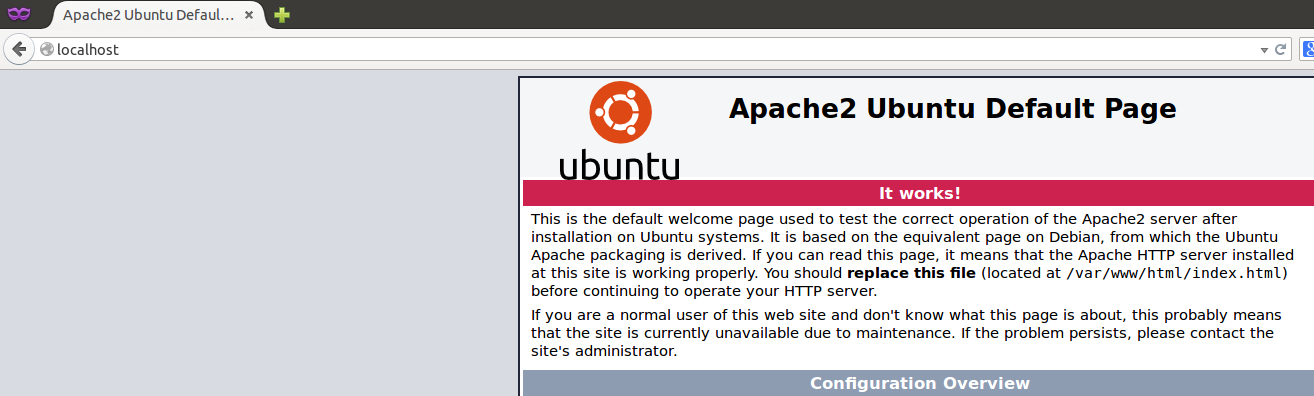
\includegraphics[width=.9\linewidth]{./media/apache-1.png}
\end{center}

Lo que se puede apreciar arriba es el por defecto.

Modificaré el fichero \texttt{.html} para que se vea con otro título y fondo

\begin{minted}[,frame=single]{css}
body, html {
  padding: 3px 3px 3px 3px;

  background-color: yellow;

  font-family: Verdana, sans-serif;
  font-size: 11pt;
  text-align: center;
}
\end{minted}

\begin{minted}[,frame=single]{html}
<body>
  <div class="main_page">
    <div class="page_header floating_element">
      <img src="/icons/ubuntu-logo.png" alt="Ubuntu Logo" class="floating_element"/>
      <span class="floating_element">
        Modificado por Maka
      </span>
\end{minted}

\begin{center}
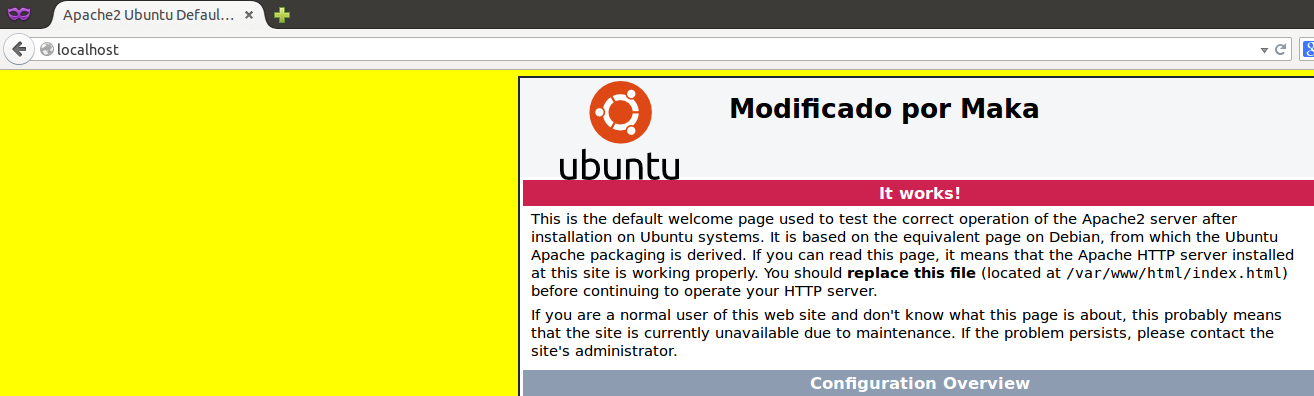
\includegraphics[width=.9\linewidth]{./media/apache-2.png}
\end{center}
\subsubsection{\emph{option indexes}}
\label{sec:org9ac6a48}
Podemos quitar la opción para ver el contenido de la siguiente forma:
\begin{enumerate}
\item Ir al fichero \texttt{/etc/apache2/apache2.conf}
\item Dónde pone \texttt{<Direcotory /var/www>}
\begin{itemize}
\item quitar el \texttt{options indexes FollowSymLinks}
\end{itemize}
\end{enumerate}
\begin{minted}[,frame=single]{html}
<Directory /var/www/>
        Options Indexes FollowSymLinks
        AllowOverride None
        Require all granted
</Directory>
\end{minted}

Ahora también tememos que cambiar el nombre del fichero \texttt{index.html} porque si no seguirá cargándolo por defecto. Luego recargaremos \texttt{apache2}
\begin{minted}[,frame=single]{bash}
root@ubuntu101:/var/www/html# mv index.html index-cambiado.html
root@ubuntu101:/var/www/html# ls -la
total 28
drwxr-xr-x 3 root root      4096 feb 19 13:12 .
drwxr-xr-x 3 root root      4096 nov  7 08:58 ..
-rw-r--r-- 1 root root     11494 feb 19 13:08 index-cambiado.html
-rw-r--r-- 1 root root        21 feb 11 09:29 prueba.php
drwxr-xr-x 2 root www-data  4096 nov  7 09:08 webmail
root@ubuntu101:/var/www/html# service apache2 reload 
 * Reloading web server apache2                                                                                             * 
\end{minted}

\begin{center}
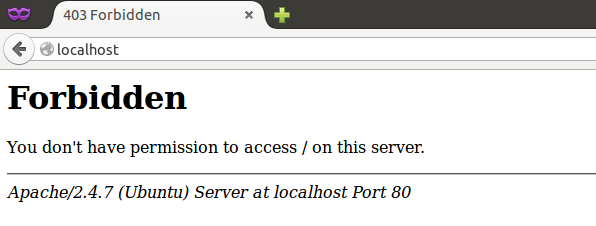
\includegraphics[width=.9\linewidth]{./media/apache-3.png}
\end{center}

Si queremos volver a habilitar esto, podemos hacerlo directamente en cada sitio de forma independiente. Añadiendolo en su sitio de configuración como por ejemplo el \texttt{000-default.conf}

Ahora volvemos a dejar todo como estaba. Como tenemos el fichero renombrado saldrá así:

\begin{center}
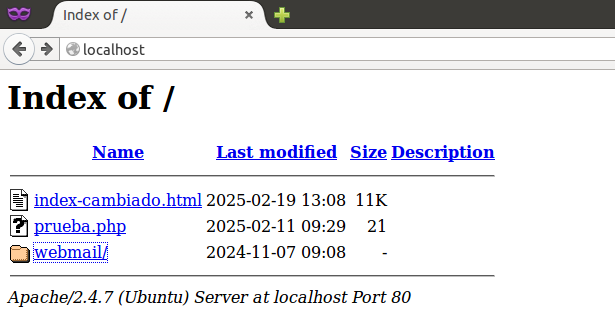
\includegraphics[width=.9\linewidth]{./media/apache-4.png}
\end{center}
\subsubsection{Crear un sitio personalizado}
\label{sec:org863732b}
Primero tendremos que crear tanto un fichero \texttt{.conf} como uno \texttt{.html}

El fichero \texttt{/etc/apache2/sites-available/sitioIsmael.conf} va a ser nuestro nuevo sitio:
\begin{minted}[,frame=single]{html}
<VirtualHost *:80>
        # The ServerName directive sets the request scheme, hostname and port that
        # the server uses to identify itself. This is used when creating
        # redirection URLs. In the context of virtual hosts, the ServerName
        # specifies what hostname must appear in the request's Host: header to
        # match this virtual host. For the default virtual host (this file) this
        # value is not decisive as it is used as a last resort host regardless.
        # However, you must set it for any further virtual host explicitly.
        ServerName www.sitioismael.com

        ServerAdmin webmaster@localhost
        DocumentRoot /var/www/sitioIsmael

        # Available loglevels: trace8, ..., trace1, debug, info, notice, warn,
        # error, crit, alert, emerg.
        # It is also possible to configure the loglevel for particular
        # modules, e.g.
        #LogLevel info ssl:warn

        <Directory /var/www/sitioismael>
                Options Indexes FollowSymLinks
                AllowOverride none
                Require all granted
        </Directory>
\end{minted}

Luego tendremos que habilitar el sitio mediante la instrucción \texttt{a2ensite} y seguidamente crearemos el fichero \texttt{.html}
\begin{itemize}
\item \texttt{sudo a2ensite sitioIsmael.conf}
\item \texttt{mkdir /var/www/sistioismael}
\item \texttt{emacs -q /var/www/sitioismael/index.html}
\end{itemize}
\begin{minted}[,frame=single]{html}
<h1>Bienvenido a www.sitioismael.com</h1>
\end{minted}

Tendremos que añadir esto al fichero \texttt{/etc/hosts}
\begin{minted}[,frame=single]{bash}
root@ubuntu101:/var/www/sitioismael# cat /etc/hosts
127.0.0.1	localhost
127.0.1.1	ubuntu1.myguest.virtualbox.org	ubuntu101
172.26.0.101	ubuntu101
192.168.9.156	www.sitioismael.com

# The following lines are desirable for IPv6 capable hosts
::1     ip6-localhost ip6-loopback
fe00::0 ip6-localnet
ff00::0 ip6-mcastprefix
ff02::1 ip6-allnodes
ff02::2 ip6-allrouters
\end{minted}

Reiniciaremos el servicio web mediante la instrucción \texttt{service apache2 reload}

\begin{center}
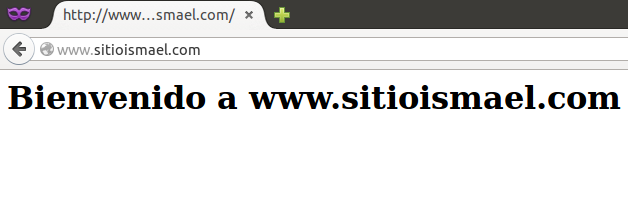
\includegraphics[width=.9\linewidth]{./media/apache-5.png}
\end{center}
\subsubsection{Contraseñas y restricción de acceso}
\label{sec:org42f0f5b}
Primero lo haremos mediante \emph{passwd-basic}, para ello tendremos que acceder al fichero \texttt{/etc/apache2/sites-enabled/sitioismael.conf}

Le pediré la autenticación para la carpeta interna que tenemos que crear después
\begin{minted}[,frame=single]{html}
<Directory /var/www/sitioismael/interna>
  AuthType basic
  AuthName "Acceso restringido a sitio interno"
  AuthBasicProvider file
  AuthUserFile /etc/apache2/passwd-basic
  Require user pedro
</Directory>
\end{minted}

Ahora tendremos que crear el usuario \texttt{pedro} de una manera un poco más especial.

\begin{alertblock}{Aviso passwd-basic}
Da igual que no exista el fichero, se crea con la instrucción htpasswd
\end{alertblock}

\begin{minted}[,frame=single]{bash}
root@ubuntu101:/var/www/sitioismael# htpasswd -c /etc/apache2/passwd-basic pedro
New password: 
Re-type new password: 
Adding password for user pedro
\end{minted}

Reiniciamos \texttt{apache2} mediante la instrucción \texttt{service apache2 reload}

\begin{center}
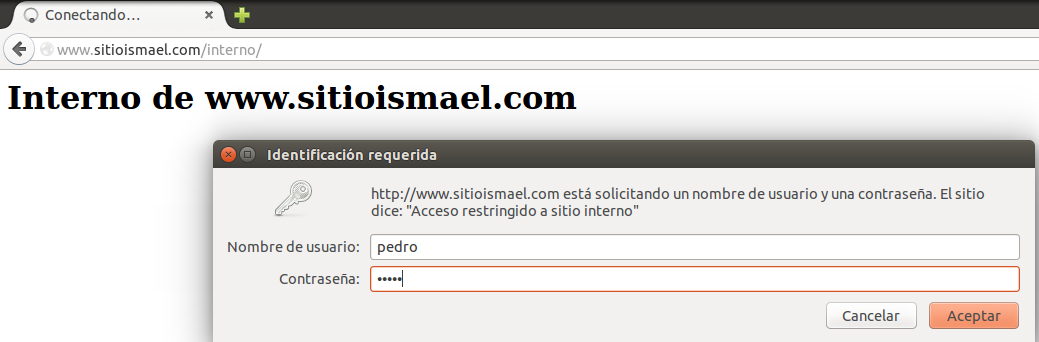
\includegraphics[width=.9\linewidth]{./media/apache-6.png}
\end{center}
\subsubsection{Páginas por puertos e IPs}
\label{sec:orgfec6a34}
Primero lo haremos mediante puertos.

Vamos a crear 2 directorios, uno para el puerto \texttt{8080}, y otro para el puerto \texttt{8081}
\begin{minted}[,frame=single]{bash}
root@ubuntu101:/var/www# mkdir puerto8080
root@ubuntu101:/var/www# mkdir puerto8081
\end{minted}

Ahora crearemos sus \texttt{sites-availables}
\begin{minted}[,frame=single]{bash}
root@ubuntu101:/etc/apache2/sites-available# cp 000-default.conf puerto8080.conf
root@ubuntu101:/etc/apache2/sites-available# cp 000-default.conf puerto8081.conf
\end{minted}

Ahora en cada uno tendremos que modificar el \texttt{VirtualHost} al puerto correspondiente de cada uno
\begin{minted}[,frame=single]{html}
<VirtualHost *:8080>
        # The ServerName directive sets the request scheme, hostname and port that
        # the server uses to identify itself. This is used when creating
        # redirection URLs. In the context of virtual hosts, the ServerName
        # specifies what hostname must appear in the request's Host: header to
        # match this virtual host. For the default virtual host (this file) this
        # value is not decisive as it is used as a last resort host regardless.
        # However, you must set it for any further virtual host explicitly.
        ServerName www.puertos.com

        ServerAdmin webmaster@localhost
        DocumentRoot /var/www/puerto8080

        <Directory /var/www/puerto8080>
                Options Indexes FollowSymLinks
                AllowOverride none
                Require all granted
        </Directory>
\end{minted}

\begin{minted}[,frame=single]{html}
<VirtualHost *:8081>
        # The ServerName directive sets the request scheme, hostname and port that
        # the server uses to identify itself. This is used when creating
        # redirection URLs. In the context of virtual hosts, the ServerName
        # specifies what hostname must appear in the request's Host: header to
        # match this virtual host. For the default virtual host (this file) this
        # value is not decisive as it is used as a last resort host regardless.
        # However, you must set it for any further virtual host explicitly.
        ServerName www.puertos.com

        ServerAdmin webmaster@localhost
        DocumentRoot /var/www/puerto8081

        <Directory /var/www/puerto8081>
                Options Indexes FollowSymLinks
                AllowOverride none
                Require all granted
        </Directory>
\end{minted}

Luego tendremos que modificar el fichero \texttt{ports.conf} de la siguiente manera
\begin{minted}[,frame=single]{bash}
# If you just change the port or add more ports here, you will likely also
# have to change the VirtualHost statement in
# /etc/apache2/sites-enabled/000-default.conf

Listen 80
Listen 8080
Listen 8081
\end{minted}

Luego habilitaremos los sitios mediante la instrucción \texttt{a2ensite}

Luego modificaremos el fichero \texttt{/etc/hosts} para que quede de la siguiente manera
\begin{minted}[,frame=single]{bash}
root@ubuntu101:/etc/apache2/sites-available# cat /etc/hosts
127.0.0.1	localhost
127.0.1.1	ubuntu1.myguest.virtualbox.org	ubuntu101
172.26.0.101	ubuntu101
192.168.9.156	www.sitioismael.com
192.168.9.156	www.puertos.com
\end{minted}

Por último, usando la instrucción \texttt{service apache2 reload} reiniciaremos el servicio web \texttt{apache}

\begin{center}
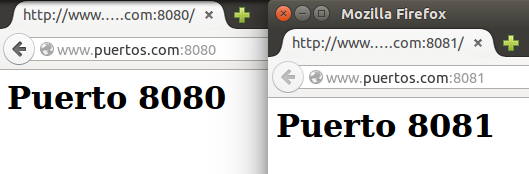
\includegraphics[width=.9\linewidth]{./media/apache-7.png}
\end{center}

Ahora lo haremos mediante la IP.

El proceso es el mismo que por puerto menos en un pequeño aspecto, en el \texttt{<VirtualHost>} en vez de tener un *, tendremos que tener la dirección IP y añadir está misma al fichero \texttt{/etc/hosts}

Primero añadiremos 2 tarjetas alías de la siguiente manera
\begin{minted}[,frame=single]{bash}
# interfaces(5) file used by ifup(8) and ifdown(8)
auto lo
iface lo inet loopback

auto eth0
allow-hotplug eth0
iface eth0 inet dhcp


auto eth0:1
allow-hotplug eth0:1
iface eth0:1 inet static
        address 10.0.1.10
        netmask 255.255.255.0

auto eth0:2
allow-hotplug eth0:2
iface eth0:2 inet static
        address 172.26.1.10
        netmask 255.255.0.0
\end{minted}

Luego de aplicar los cambios y verlos reflejados a través de la instrucción \texttt{ip a} ya podremos modificar los fichero \texttt{/etc/apache2/sites-available/puerto8080.conf}
\begin{minted}[,frame=single]{html}
<VirtualHost 10.0.1.10:8080>
        # The ServerName directive sets the request scheme, hostname and port that
        # the server uses to identify itself. This is used when creating
        # redirection URLs. In the context of virtual hosts, the ServerName
        # specifies what hostname must appear in the request's Host: header to
        # match this virtual host. For the default virtual host (this file) this
        # value is not decisive as it is used as a last resort host regardless.
        # However, you must set it for any further virtual host explicitly.
        ServerName www.puertos.com

        ServerAdmin webmaster@localhost
        DocumentRoot /var/www/puerto8080

        <Directory /var/www/puerto8080>
                Options Indexes FollowSymLinks
                AllowOverride none
                Require all granted
        </Directory>
\end{minted}

\begin{minted}[,frame=single]{html}
<VirtualHost 172.26.1.10:8081>
        # The ServerName directive sets the request scheme, hostname and port that
        # the server uses to identify itself. This is used when creating
        # redirection URLs. In the context of virtual hosts, the ServerName
        # specifies what hostname must appear in the request's Host: header to
        # match this virtual host. For the default virtual host (this file) this
        # value is not decisive as it is used as a last resort host regardless.
        # However, you must set it for any further virtual host explicitly.
        ServerName www.puertos.com

        ServerAdmin webmaster@localhost
        DocumentRoot /var/www/puerto8081

        <Directory /var/www/puerto8081>
                Options Indexes FollowSymLinks
                AllowOverride none
                Require all granted
        </Directory>
\end{minted}

\begin{center}
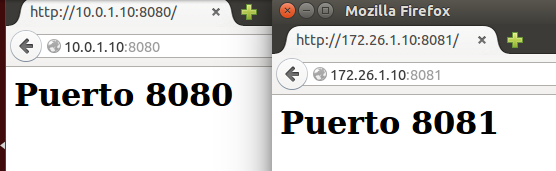
\includegraphics[width=.9\linewidth]{./media/apache-8.png}
\end{center}
\subsubsection{Sitio virtual, directorios \emph{userdir}}
\label{sec:orge41505e}
Para esto comenzaremos como siempre, creando un fichero en \texttt{sites-available}, en este caso se llamará \texttt{arbol.conf}
\begin{minted}[,frame=single]{html}
<VirtualHost *:80>
        # The ServerName directive sets the request scheme, hostname and port that
        # the server uses to identify itself. This is used when creating
        # redirection URLs. In the context of virtual hosts, the ServerName
        # specifies what hostname must appear in the request's Host: header to
        # match this virtual host. For the default virtual host (this file) this
        # value is not decisive as it is used as a last resort host regardless.
        # However, you must set it for any further virtual host explicitly.
        ServerName www.arbol.com

        ServerAdmin webmaster@localhost
        DocumentRoot /var/www/arbol

        <Directory /var/www/puerto8080>
                Options Indexes FollowSymLinks
                AllowOverride none
                Require all granted
        </Directory>
        # Available loglevels: trace8, ..., trace1, debug, info, notice, warn,
        # error, crit, alert, emerg.
        # It is also possible to configure the loglevel for particular
        # modules, e.g.
        #LogLevel info ssl:warn

        ErrorLog ${APACHE_LOG_DIR}/error.log
        CustomLog ${APACHE_LOG_DIR}/access.log combined
        UserDir public_html
\end{minted}

Ahora tenemos que habilitar tanto el sitio como el módulo \texttt{userdir} mediante las siguientes instrucciones:
\begin{itemize}
\item \texttt{a2ensite arbol.conf}
\item \texttt{a2enmod userdir}
\end{itemize}

\begin{minted}[,frame=single]{html}
<IfModule mod_userdir.c>
        UserDir public_html
        UserDir disabled root

        <Directory /home/*/public_html>
                AllowOverride FileInfo AuthConfig Limit Indexes
                Options MultiViews Indexes SymLinksIfOwnerMatch IncludesNoExec
                <Limit GET POST OPTIONS>
                        Require all granted
                </Limit>
                <LimitExcept GET POST OPTIONS>
                        Require all denied
                </LimitExcept>
        </Directory>
</IfModule>

# vim: syntax=apache ts=4 sw=4 sts=4 sr noet
\end{minted}

Lo siguiente sería crear en la carpeta de la \texttt{\$HOME} una carpeta \texttt{public-html} con un fichero \texttt{.html} de la siguiente manera:
\begin{itemize}
\item \texttt{mkdir /home/maka/public-html}
\item \texttt{echo "<h1>Mi PAGINA DE MAKA</h1>" > /home/maka/public-html/index.html}
\end{itemize}

Luego de esto solo faltaría modificar el fichero \texttt{/etc/hosts} de la siguiente manera
\begin{minted}[,frame=single]{bash}
127.0.0.1       localhost
127.0.1.1       ubuntu1.myguest.virtualbox.org  ubuntu101
172.26.0.101    ubuntu101
192.168.9.156   www.sitioismael.com
192.168.9.156   www.puertos.com
192.168.9.156   www.arbol.com
\end{minted}
\subsubsection{Securización}
\label{sec:org4ef3afe}
Simplemente tendremos que habilitar el sitio \texttt{/etc/apache2/sites-available/default-ssl,conf} y el módulo \texttt{ssl} con las siguientes instrucciones:
\begin{itemize}
\item \texttt{a2ensite default-ssl.conf}
\item \texttt{a2enmod ssl}
\item \texttt{sudo service apache2 reload}
\end{itemize}
\end{document}
